\documentclass[times,12pt]{article}
\usepackage{amsmath,amssymb,amsthm,mathrsfs,graphicx}
\usepackage{titlesec}
\usepackage{algorithm}
\usepackage{color}
\usepackage{float}
\usepackage{graphicx}
\usepackage{rotating}
\usepackage{url}
\usepackage{fancyhdr}

\usepackage{algorithmicx, algorithm, algpseudocode}
\floatname{algorithm}{Algorithm}

\pagenumbering{arabic}

\setlength{\parindent}{0pt}
\setlength{\parskip}{5pt plus 2pt minus 1 pt}

\topmargin  -15mm
\evensidemargin 0mm
\oddsidemargin  0mm
\textwidth  160mm
\textheight 235mm
\frenchspacing
\sloppy
\titlespacing{\section}{0pt}{\parskip}{0.01\parskip}
%%%%%%%%%%%%%%%%%%%%%%%%%%%%%%%%%%%%%%%%%%%%%%%%%%%%%%%%%%%%%%%%%%%%%%%

\begin {document}

\pagestyle{plain}

\begin{center}
{\fontsize{22}{20}\bf A Parallel Grid-based Approach for Multiscale Non-Spherical Geometry Impact Dynamics\\
}\end{center}

\vspace{\fill}
\begin{center}\fontsize{16}{20}
\textbf{Konstantinos Krestenitis$^1$}\\
\today
\end{center}
\vspace{\fill}

\begin{center}
{\fontsize{10}{12}
}\end{center}

\begin{center}
$^1$School of Engineering and Computing Sciences, University of Durham, DH1 3LE, Durham\\
konstantinos.krestenitis@durham.ac.uk\\
Mechanics Research Group\\
\end{center}
\begin{center}
Supervised by\\
Dr Tobias Weinzierl\\
Dr Tomasz Koziara (former)\\
Professor Jon Trevelyan\\
\end{center}

\clearpage

\tableofcontents

\clearpage

\section{Introduction}
We present a Discrete Element Method (DEM) contact detection code that simulates rigid non-spherical particles on manycore shared memory machines and distributed memory computers. DEM is used to study granular particles in fields like soil mechanics. We rely on triangulated particle meshes to model surfaces. Spherical or multi-sphere models currently are state-of-the-art - due to a lack of well-suited software and runtime demands. Non-spherical particles promise to facilitate more accurate physics than sphere-based approaches \cite{AlonsoMarroqu2013}. The focus on triangles for rigid contact mechanics facilitates memory layouts allowing vectorised computation \cite{Alvarez2007, Koziara2005, Krestenitis2015}. It is vital to yield high performance on current and upcoming processor architectures to enable engineers to simulate more realistic materials.

It is important to investigate the problem of finding the minimum distance between triangles because of the changes in the computational hardware \cite{Dongarra2011}. The central processing unit architecture today and the future upcoming hardware support Single Instruction Multiple Data (SIMD)\cite{Alvarez2007} parallelism which allow data level parallelism. These speed-ups are enabled because of new instruction sets and wide vector register. Furthermore, shared memory parallelism at the node level as well as distributed memory for supercomputers can provide significant speed-ups. It is vital to extract resources available on current and upcoming hardware, the speed-ups enable more triangles to be used to describe surfaces. Consequently, our objective is to enable engineers to use an algorithm that is capable to handle the maximum amount of triangles per time step to do better engineering and science.

In the present work we propose a hybrid method that combines the advantages of two optimised triangle-to-triangle distance computation methods. It benefits from both performance and robustness of an iterative Newton-penalty and a brute force solver. We exploit shared memory parallelism and SIMD (Single Instruction Data) to perform contact detection at the node level. On distributed memory, we use spatial domain decomposition  whilst with the Message Passing Interface (MPI), we exploit asynchronous non-blocking communication to overlap data exchange with computation.

The state-of-the-art large scale DEM work, to the best of my knowledge, relies on sphere-based or multi-sphere particles \cite{Gonnet2013, Gonnet2014}. Large scale applications of spherical particles can be found in the field of molecular dynamics. Large scale non-spherical particle based DEM simulations in literature \cite{Girolami2012, Iglberger2009, Iglberger2010, Iglberger2011} often describe particles as convex polyhedra and contact detection is resolved with GJK (Gilbert-Johnson-Keerthi) \cite{Ericson2005} variants which require interpenetration and access to all vertices of the particle to detect contact on the surface. Interpenetration introduces contact point clustering and the problem of divergence \cite{Koziara2008, koziara2011, Krestenitis2015}. In addition, convex polyhedra based contact detection methods require undeterministic memory access to all particle simplices \cite{Ericson2005} which is contradictory to the aligned memory access imposed by SIMD for data locality. Triangle-based contact detection retain locality for vectorisation as well as increases accuracy of contact point generation \cite{Krestenitis2015}. Furthermore, the method can be extended to run on shared memory manycore and distributed memory machines.

The remainder of the paper is structured as follows. In Section 2, we describe the serial DEM  algorithm. In Section 3 we review two triangle-to-triangle distance algorithms. We create a new hybrid shared memory method that benefits from fast convergence and robustness. Next, in Section 3, we propose a distributed memory algorithm for contact detection that use asynchronous communication to overlap computation over communication. Section 4, discusses the future research directions.

\section{Outline Summary of Thesis}

\subsection{Overview}

In contact mechanics, fluid-stucture interaction or other fields, it is an essential task to compute the distance between geometries to determine contact. Contact detection also is the most expensive algorithmic step \cite{Koziara2010, Wachs2012}. We present a Discrete Element Method (DEM) code that simulate particles that interact with spring-based contact. Non-spherical particles promise to facilitate more accurate physics than sphere-based approaches \cite{AlonsoMarroqu2013, Girolami2012}. The contact detection routine determines contact based on the distance between the triangles of every particle against all other. If two triangles are closer than a prescribed threshold, they are considered to contact each other. The use of triangles for rigid body contact dynamics rather than arbitrary polygons simplifies geometric checks and facilitates memory layouts that allow vectorised computation \cite{Eichenberger2004, Juurlink, Krestenitis2015, Krestenitis2016}.

\subsubsection{Geometric Approximation}

In this section, i go through the use of geometric elements in 3D that approximate simulated rigid body dynamics. According to literature [][][][] spherical elements are the most widely used in DEM simulations. In the thesis i will review multiple elements (sphere, multispheres, ellipsoids) to approximate non-spherical geometries. The element chosen to describe the arbitrary surface of solid bodies affects the geometric approximation, interaction model, particle volume, inertia properties, and resulting simulation overall.

For the research project, i chose to increase the geometric approximation by inserting triangulated surfaces from CAD models, or point clouds of non-spherical solids. Reducing geometric error according to the literature [][] promises to increase the accuracy of predicting physical phenomena in simulations. But reducing the approximation error is not free as the computational cost is increased; this is discussed in the algorithmic chapter. 

\subsubsection{Interaction Model}

This section reviews the interaction model used in DEM simulations in literature and in the project. There are four stages that are fundamental to simulate interactions; contact detection, contact point definition, time integration, force derivation. In my thesis i focus in contact detection and contact point generation for non-spherical rigid body interactions.  

\begin{algorithm}	
  \textbf{\textcolor{blue}{FUNCTION}} f = Force(normal, relativeVelocity, depth, massA, massB)
  
  1~~mass = 1.0 / ((1/massA) + (1/massB));
  
  2~~velocitymagnitude = DOT(relativeVelocity, normal);
  
  3~~magnitude = SPRING*depth + DAMPER*sqrt(SPRING*mass)*velocitymagnitude;
  
  4~~force = magnitude*normal;
  
  \textbf{\textcolor{blue}{ENDFUNCTION}}
\protect\caption{\label{forceDashpot}Spring-dashpot force algorithm}
\end{algorithm}

The forces in DEM are modelled with the spring-dashpot model \cite{Koziara2008, solberg2000, Wachs2012, Williams1999}. Algorithm \ref{forceDashpot} shows the spring-dashpot force approach. Where using the contact point normal, mass, relative particle velocity we get a force. Augmentations of spring-dashpot can accommodate multiple physical phenomena like friction, adhesiveness, force fields. 

As a prerequisite to force derivation it is vital to estimate the distance between interaction pairs [] to derive forces. For this i discuss about three newly created models for computing the distance between triangles. The three solvers differ in terms of numerical approximation error and in terms of algorithmic characteristics for parallel processing and memory footprint. In addition i will review available literature on the subject and validate my model against existing methods for non-spherical particle contact detection and point generation. []  

Using the distance derived we define a unique point of contact and the artificial interpenetration depth to compute force normal and magnitude. For arbitrary shaped non-spherical particles this process can become more complex than in spherical particles as multiple contacts can occur in one pair in addition to having redundant points due to mesh refinement over a surface area. 
    
Parameter studies for stiffness and damping were not rigorously studied. But a new damping model for non-spherical particle was derived with T.Koziara [] and it is discussed in detail in the thesis as it is significant improvement for energy dissipation of static bodies with angular velocity oscillations/vibrations over surfaces.   


\subsection{Algorithmic Overview}

The algorithmic sequence is discussed in detail to demonstrate to evolution of a serial DEM code into a scalable parallel code. The discussion is based on three pillar concepts; computational hotspots, data locality/communication, theoretical peak performance. Based on those principles the DEM code is evolved into a scalable parallel code.
 
\begin{algorithm}	

1 \textbf{\textcolor{blue}{FOR}} time = 0; time $<$ simulation time; time+=step

2~~~//contact detection
		
3~~~~~~	\textbf{\textcolor{blue}{FOR}} i = 0 to N triangles

4~~~~~~~~~\textbf{\textcolor{blue}{FOR}} j = i+1 to N triangles
				
5~~~~~~~~~~~~distance = TTD(i,j)
				
6~~~~~~~~~~~~\textbf{\textcolor{blue}{IF}} (distance $<$ margin) AND ParticleID(i) != ParticleID(j)

7~~~~~~~~~~~~~~~contact(PID(i)).add(point, normal)

8~~~~~~~~~~~\textbf{\textcolor{blue}{ENDIF}}
			
9~~~~~~~~~\textbf{\textcolor{blue}{	ENDFOR}}
			
10~~~~~~\textbf{\textcolor{blue}{ENDFOR}}

11~~~//force derivation
		
12~~~~~~\textbf{\textcolor{blue}{FOR}} z = 0 to NB particles

13~~~~~~~~~	\textbf{\textcolor{blue}{FOR}} k = 0 to contacts(z).size()

14~~~~~~~~~~~~~~~force = granular(velocity(z), position(z), contacts(z).getcontact(k))

15~~~~~~~~~	\textbf{\textcolor{blue}{ENDFOR}}

16~~~~~~\textbf{\textcolor{blue}{ENDFOR}}
	
17~~~//explicit time integration

18 \textbf{\textcolor{blue}{ENDFOR}}

\protect\caption{\label{algorithmPseudo}DEM Serial Pseudo code}
\end{algorithm}

The Algorithm \ref{algorithmPseudo} demonstrates the execution sequence of DEM. The contact detection stage has a O($n^2$) complexity at the lowest level of element decomposition (each particle is decomposed into triangular elements). At line 3 and line 4 the nested for loop indicate the complexity of iterating through all triangle pairs. At line 5 TTD(i, j) invokes a Triangle-to-Triangle Distance (TTD) algorithm that determines the distance between triangle i and triangle j. Based on the boundary layer margin contact model \cite{Krestenitis2015} to avoid penetration, we check whether distance between Triangle i and j is smaller than a set margin (line 6). If the parent particle of triangle i and j is not the same then this indicate a contact point between the two particles (line 7). The contact point information at line 13 and line 14 is used to derive the forces. The forces derivation and Euler explicit time integration stages define the interaction. 

First we discuss the hotspots of the code, which based on complexity studies and experimental validation lye on the contact detection stage. To reduce the hotspot we attempt to reduce the overall algorithmic complexity by space decomposition, adaptivity and utilization of multiple parallel computational paradigms. I cover two paradigms in the Flynn taxonomy Single Instruction Multiple Data (SIMD), Single Program Multiple Data (SPMD) and three levels of simultaneous parallelism. At the finest granularity i exploit instruction level pipe-lining on a single core. Then concurrent multi-threading (SMT) is applied to allocate workload to cores on a single compute node. Furthermore distributed memory is discussed (SPMD) and implications of communication between processes.

\subsubsection{Space Decomposition}

Space decomposition chapter is focusing on the utilisation of techniques to reduce the overal complexity of the algorithm while providing dense arithmetic locality, intensity to the cores. Decomposition is investigated in two chapters, structured and unstructured data and space decomposition. Both approaches have implications in communication, all levels of computation. 

For unstructured domain decomposition space is divided into subdomains using the recursive bisection (RCB) method where points are mapped int a kd-tree variant in the computational space. This ensures load balancing stability at all times but at the cost of recursive refinement and non-aligned memory mapping. On the other hand, i discuss that structured domain decomposition offers greater locality, memory alignment. As the refinement level is located at the particle level the produced tree mapping (quadtree) is shorter than point level and the levels are more deterministic. In addition a uniform structured space decomposition provides better communication scalability.  

\subsubsection{Vectorisation}

Vectorisation covers the techniques utilised to efficiently optimize the computation. The section covers memory layout requirements and code practices in HPC. A discussion about structure of arrays (SoA) and array of structures (AoS) and their implication on SIMD as well as cache. Other optimization techniques discussed fall into loop analysis; loop fusion, memory alignment, loop unrolling, loop splitting, loop unswitching.

\subsubsection{Shared Memory}

In the shared memory chapter, i discuss three levels of shared memory implementations; mesh level parallelism, particle level and cell level. All three levels are discussed as well as the interplay of physical space and computational space. The physical space can trigger different hotspots at multiple levels of parallelism affecting the arithmetic intensity of each thread. That means dense tessellation of the mesh, dense particle arrangements, and multi-clustered particle arrangements have all different shared memory characteristics and has implications to the locality of reference and granularity of threading. Moreover, topics covered are implementation techniques like ccNUMA awareness, thread level load balancing, arithmetic granularity. 

\subsubsection{Distributed Memory}

In chapter distributed memory computation, i cover the feeding of compute nodes with dense arithmetic operations, communication behaviour in different load balancers and grid frameworks.
For non-uniform space decomposition i show techniques that overlap computation with communication but also scalability studies that prove the method is ineffective for large scale DEM applications. The report will include uniform structured space decomposition scalability measurements and communication pattern that emerge in large scale multiscale DEM simulations. 

\subsection{Case Study}

In this research project we implement multiple case studies to validate numerical stability and perform performance benchmarks. Relying on two engineering application we explore two contrasting scenarios; flow of non-spherical granulates from a hopper structure and low oscillatory vibrations of a nuclear reactor assembly on a shaking table. The case study investigate and validate the behaviour geometric approximation the affect it has on the physics domain, the interplay of data communication within a level of paralelism (shared memory, distributed memory), grid adaptivity behaviour, FLOPs-memory benchmarks.

\subsubsection{Hopper Flow}

The hopper scenario involves a hopper structure placed above a ground. Hopper scenarios are found in process engineering and manufacturing in geo-technical and pharmaceutical industry []. An important process is filtering and sorting granular particles of different shapes and size by tracking their physical geometry, moment of inertia.

In phase one, multi scale spherical particles are placed above the hopper structure, gravity is applied and they are allowed to fall through the structure. In phase two we rerun the same experiment but with non-spherical particles. Data about the simulation of each particle kinematics and interaction is stored. Phase one and phase two is compared to experimentally validate the difference in geometric approximation and increase in physics quality.

\subsubsection{Seismic Shake}

In the second scenario we import the geometry of a single array Advanced Gas Cooled nuclear reactor onto a artificial shaking table. The shaking table simulates the physical seismic shaking table of earthquake analysis labs. In my case study to keep engineering simple i do not thoroughly study shaking tables that induce more than one degrees of freedom to the stressed structure. Again as in the hopper scenario i showcase how the computational domain and its underlying domain is 
mapped into the hardware. Geometric approximation error is again important and spherical DEM has higher error and experimental studies show [] that these errors propagate from the kinematics studies into elasticity, fracture simulations due to the interdependency between them in a complete seismic numerical/computational experiment.

\section{Progress Report}

\subsubsection{Overview}



\subsubsection{Geometric Approximation}

Unlike conventional large scale DEM frameworks that use spherical particles [][][], we choose to increase the surface approximation of our simulated geometries by using non-spherical particles to simulate non-spherical interactions. According to experimental studies [] in DEM, the surface can affect the interaction physics thus the results. In the case of using spheres to describe particles that are not spherical particles, approximation of properties like mass, torque, moment of inertia is not possible. Interactions between spherical particles that approximate the geometry, properties and interaction behaviour of non-spherical particles cannot be captured in the simulated environment without some degree of error []. 

Coarse particle applications that require non-spherical particle surface can be found in process engineering, seismic engineering, manufacturing, etc []. Due to the computational time and error of approximation trade off it is widely accepted to compromise on the geometric approximation depending on applications where capturing macroscopic phenomena can be sufficient []. Multisphere particles are reducing the error of approximation and improve the capture of properties like inertia, mass and angular velocity phenomena [].   

For the library, we primarily use non-spherical particles as with numerical modelling and computational optimizations it possible to close the gap in geometric approximation trade off. Spherical particles are used to validate their different behaviour against non-spherical particles experimentally in case studies. To create granular geometries for the simulations we utilise particles approximated by a random spherical point cloud, surfaces are generated with the convex hull and Delauny triangulation algorithm. For experimental purposes we can adjust the irregularity of granular particles, radius and the mesh density. For pre-designed CAD geometries we can import the mesh directly into the simulation domain. 

\begin{figure}[!h]
\centering
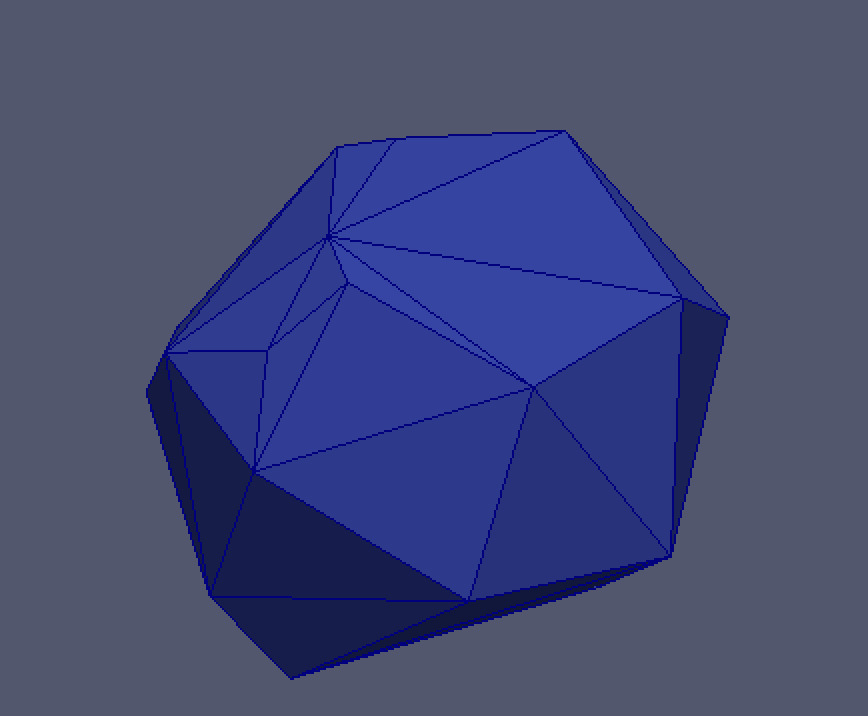
\includegraphics[width=0.5\textwidth]{sketches/coarse.png} \protect\caption{\label{granulate} A coarse surface granulate generated with convex hull algorithm.}
\end{figure} 


\subsubsection{Interaction Model}

Other than the implementation of the DEM model for kinematics; force derivation, damping coefficient, static friction, rolling friction, torque, angular/linear velocities, mass, moment of inertia matrix computation, rotation matrix, time integration, and contact normals computation, the focus of research is in the computational hotspot of interactions. The contact detection stage is modelled with the introduction of two new numerical models; the brute force and the Newton-penalty methods. Both methods challenge current contact point determination numerical models of arbitrary convex and non-convex polyhedra geometries[]. 

%Brute Force
The brute force is the naive approach to contact detection, it computes all distances between geometrical primitives of the triangles. The method computes the distance between all line segments of one triangle with the line segments of the other using the segment-to-segment (Algorithm \ref{alg3}, line 22-30) distance function \cite{Ericson2005, Tropp2006}. Then for every point of one triangle it computes the distance against the other triangle using the point-to-triangle (Algorithm \ref{alg3}, line 3-8) function \cite{Eberly1999, Ericson2005}. The method requires evaluating the minimum distance among all comparisons performed to find the overall minimum distance in the end.

The algorithm is straight-forward because it relies on only two geometric comparisons. As seen in Algorithm \ref{alg3} in lines 3 to 21 the six comparisons yield one that defines the distance. For segment-to-segment, let $v_{1i}$, $e_{1i}$, $v_{2i}$, $e_{2i}$ be the vertices and edges of triangles $T_1$ and $T_2$. The brute force approach computes all fifteen distances $v_{1i}$-to-$T_2$, $v_{2i}$-to-$T_1$, $e_{1i}$-to-$e_{2i}$, and then we select the shortest distance. As seen in Algorithm \ref{alg3} in line 22 to 37 the algorithm determines the segment-to-segment distance between all segments of the triangle pair. Finally the algorithms finds the minimum of the two sets of comparisons to get the P and Q vertices that define the distance between two triangles. 

Optimization of the brute force method can at most rely on avoiding redundant evaluations parts of the computation. It is not possible to avoid logical branching because we have to evaluate all if statements to arrive to the solution. Therefore it is not possible to optimize the method for SIMD parallelism because of the branching. 

\begin{algorithm}
0~~\textbf{\textcolor{blue}{FUNCTION}} [min,P,Q] = \textbf{\textcolor{blue}{bf}}(A,B,C, D,E,F)

1~~T1=[A;B;C;];~~T2=[D;E;F;];

3~~[ptlist(1), P0(1,:)]= pt([D;E;F], T1(1,:));

4~~[ptlist(2), P0(2,:)]= pt([D;E;F], T1(2,:));

5~~[ptlist(3), P0(3,:)]= pt([D;E;F], T1(3,:));

6~~[ptlist(4), P0(4,:)]= pt([A;B;C], T2(1,:));

7~~[ptlist(5), P0(5,:)]= pt([A;B;C], T2(2,:));

8~~[ptlist(6), P0(6,:)]= pt([A;B;C], T2(3,:));

9~~ptmin = min(ptlist);

10~~\textbf{\textcolor{blue}{FOR}} i=1:6

11~~~~\textbf{\textcolor{blue}{IF}}(ptmin==ptlist(i))

12~~~~~~\textbf{\textcolor{blue}{IF}}(i<4)

13~~~~~~~~p1 = T1(i,:);~~p2 = P0(i,:);

15~~~~~~\textbf{\textcolor{blue}{ELSE}}

16~~~~~~~~p1 = P0(i,:);~~p2 = T2(i-3,:);

18~~~~~~\textbf{\textcolor{blue}{END;}}~~\textbf{\textcolor{blue}{break;}}

20~~~~\textbf{\textcolor{blue}{END;}}

21~~\textbf{\textcolor{blue}{END;}}

22~~[ss(1),sp1(1,:),sp2(1,:)]=segseg(T1(1,:),T1(2,:),T2(1,:),T2(2,:));

23~~[ss(2),sp1(2,:),sp2(2,:)]=segseg(T1(1,:),T1(2,:),T2(2,:),T2(3,:));

24~~[ss(3),sp1(3,:),sp2(3,:)]=segseg(T1(1,:),T1(2,:),T2(3,:),T2(1,:));

25~~[ss(4),sp1(4,:),sp2(4,:)]=segseg(T1(2,:),T1(3,:),T2(1,:),T2(2,:));

26~~[ss(5),sp1(5,:),sp2(5,:)]=segseg(T1(2,:),T1(3,:),T2(2,:),T2(3,:));

27~~[ss(6),sp1(6,:),sp2(6,:)]=segseg(T1(2,:),T1(3,:),T2(3,:),T2(1,:));

28~~[ss(7),sp1(7,:),sp2(7,:)]=segseg(T1(3,:),T1(1,:),T2(1,:),T2(2,:));

29~~[ss(8),sp1(8,:),sp2(8,:)]=segseg(T1(3,:),T1(1,:),T2(2,:),T2(3,:));

30~~[ss(9),sp1(9,:),sp2(9,:)]=segseg(T1(3,:),T1(1,:),T2(3,:),T2(1,:));

31~~ssmin = min(ss);

32~~\textbf{\textcolor{blue}{FOR}} i=1:9

33~~~~\textbf{\textcolor{blue}{IF}}(sslist(i) == ssmin)

34~~~~~~csp1 = sp1(i,:);~~csp2 = sp2(i,:);

36~~~~\textbf{\textcolor{blue}{END;}}

37~~\textbf{\textcolor{blue}{END;}}

38~~min = min(ssmin, ptmin);

39~~\textbf{\textcolor{blue}{IF}} min == ptmin

40~~~~P = p1;~~Q = p2;

41~~\textbf{\textcolor{blue}{ELSEIF}} min == ssmin

42~~~~P = csp1(:,:);~~Q = csp2(:,:);

43~~\textbf{\textcolor{blue}{END;}}
\protect\caption{\label{alg3}MATLAB Brute Force Solver.}
\end{algorithm}
\clearpage

%Penalty

The second approach to solve the triangle-to-triangle  distance problem is by parameterising of the triangles such that the distance between them is formulated by a quadratic function and a solvable minimization problem. This approach is iterative compared to brute force. The method approximate the solution using Newton iterations.

The method relies on an optimization-based formulation of the distance between two points. Let $x$ and $y$ be two points, belonging respectively to triangle $T_1$ and $T_2$. Assuming that points $A, B, C$ are vertices of $T_1$ and that points $D, E, F$ are vertices of $T_2$, $x$ and $y$ can be defined using the following equations: 
\begin{align*}
T_{1}:x(a,b)=A+(B-A) \cdot a+(C-A)\cdot b
\end{align*}
\begin{align*}
T_{2}:y(g,d)=D+(E-D) \cdot g+(F-D) \cdot d
\end{align*} 
To find the minimum distance between $T_1$ and $T_2$ and the corresponding two closest points $P$, $Q$ on the two triangles we minimize
\begin{align*}
f\left(a,b,c,d\right)=\left\Vert x\left(a,b\right)-y\left(c,d\right)\right\Vert ^{2}
\end{align*} 

What has to be noted is that $x$ and $y$ have to stay within the area of the two triangles. The four parameters of the function $f$ have to comply with six inequality constraints:
\begin{align*}
min_{a,b,g,d} f(a,b,g,d)
\end{align*}  
$$such \:that: \: \{a\geq0,b\geq0, a+b\leq1, d\geq0, g\geq0, g+d\leq1 \}$$ 

\begin{figure}[!h]
\centering
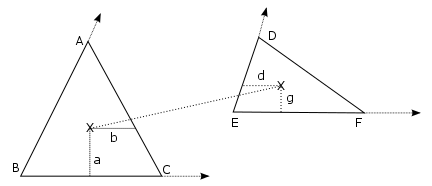
\includegraphics[width=0.6\textwidth]{c} \protect\caption{\label{fig1}Example of minimum distance and the corresponding barycentric points (parameters of objective function) on a pair of triangles in 3D. Triangle X:T1 has points A, B, C where barymetric parameters a,b correspond to point $x$ on the triangle. Triangle Y:T2 has points D,E,F where barymetric parameters g,d correspond to a point $x$. The two defined barymetric points define the minimum distance between the two triangles in 3D.}
\end{figure} 

To find the minimum of the parabolic constraint problem the Newton-Raphson method is used. Newton method use information from the curvature of the problem using the Hessian and gradient to arrive to a minimum point. To enforce the constraints the problem is transformed into a series of unconstrained problems with the augmentation of the objective function $f$ using the penalty-based method.

The penalty function penalizes the iteration so that the boundaries of the feasible region are valid; at least in a weak sense. Although there are factors that determine the number of iterations required the tuned-to-the-problem parameters yield a good number of Newton iterations that cannot be reduced to less than two; (initial guess to penalized boundary step, correction step).

\begin{figure}[!h]
\centering
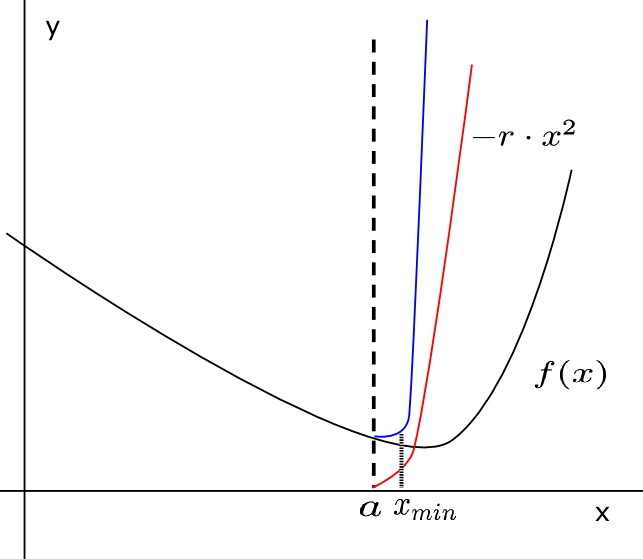
\includegraphics[width=0.5\textwidth]{penalty} \protect\caption{\label{fig2}Illustration of a 2D problem showing the penalty function (red line) penalizing the objective function (black line) f(x) under a constraint $a$ (dash line) to create the feasible region (blue line).}
\end{figure} 

This iterative approach adds a penalty term to the objective function to penalize the solution when outside of the feasible region: 
\begin{equation}\label{eq:penalty}
P(x)=f(x)+r\sum_{i=1...6}max(0,c(x_{i}))^{2}
\end{equation}
Where r is the penalty parameter (Figure \ref{fig2}). Newton iterations always converge to a solution slightly on the outside of the feasible region. Convergence can be controlled by the r penalty parameter that controls the sharpness of the curve for the constraints. One aspect that requires care however is the invertibility of the Hessian $\nabla\nabla P$. 

Furthermore that the problem is ill conditioned and a Quasi-Newton method has to be used. The Hessian matrix is not invertible so it is not possible to solve the direction of the search by computing the Hessian and gradient. This illustrates the fact that $f$ has multiple minima and $\nabla\nabla f$ is singular. Consequently, $\nabla\nabla P$ is also singular inside of the feasible region. The ill conditioning is caused by the problem definition itself, where there is a state where there are multiple solutions to the problem based on the orientation of the two triangles. This is also revealed by the two zero eigenvalues of the Hessian. Because of the ill-conditioning, we use a quasi-Newton approach, where the Hessian is approximated by a perturbed operator $\nabla\nabla P + \epsilon I$. $I$ is an identity matrix and $\epsilon$ is suitably small. 

\begin{algorithm}
0~~\textbf{\textcolor{blue}{FUNCTION}}~x~=~\textbf{penalty}(A,~B,~C,~D,~E,~F,~rho,~tol)

1~~BA~=~B-A;~CA~=~C-A;~ED~=~E-D;~FD~=~F-D;

2~~hf~=~{[}2{*}BA{*}BA',~2{*}CA{*}BA',-2{*}ED{*}BA',-2{*}FD{*}BA';

3~~~~~~~~2{*}BA{*}CA',~2{*}CA{*}CA',-2{*}ED{*}CA',-2{*}FD{*}CA';

4~~~~~~~-2{*}BA{*}ED',-2{*}CA{*}ED',~2{*}ED{*}ED',~2{*}FD{*}ED';

5~~~~~~~-2{*}BA{*}FD',-2{*}CA{*}FD',~2{*}ED{*}FD',~2{*}FD{*}FD'{]};

6~~x~=~{[}0.33;~0.33;~0.33;~0.33{]};

3~~\textbf{\textcolor{blue}{FOR}}~i=1:99

4~~~~X~=~A+BA{*}x(1)~+~CA{*}x(2);

5~~~~Y~=~D+ED{*}x(3)~+~FD{*}x(4);

6~~~~gf~=~{[}2{*}(X-Y){*}BA';~2{*}(X-Y){*}CA';~-2{*}(X-Y){*}ED';~-2{*}(X-Y){*}FD'{]};~

7~~~~h~=~{[}-x(1);~-x(2);~x(1)+x(2)-1;~-x(3);~-x(4);~x(3)+x(4)-1{]};

8~~~~dh~=~{[}-1,~0,~1,~0,~0,~0;~0,~-1,~1,~0,~0,~0;

9~~~~~~~~~~~0,~0,~0,~-1,~0,~1;~0,~0,~0,~0,~-1,~1{]};

10~~~mask~=~h'~$>$=~0;

11~~~dmax~=~dh.{*}~{[}mask;~mask;~mask;~mask{]};

12~~~gra~=~gf~+~rho~{*}~dmax~{*}~max(0,h(:));

17~~~hes~=~hf~+~rho{*}dmax{*}dmax'~+~eye(4,4)/rho\textasciicircum{}2;

18~~~dx~=~hes\textbackslash{}gra;

19~~~DX~=~BA{*}dx(1)~+~CA{*}dx(2);

20~~~DY~=~ED{*}dx(3)~+~FD{*}dx(4);

21~~~error~=~sqrt(DX{*}DX'+DY{*}DY');

22~~~\textbf{\textcolor{blue}{IF}}~error~$<$~tol,~\textbf{\textcolor{blue}{BREAK}};~\textbf{\textcolor{blue}{END}}

23~~~x~=~x~-~dx;

24~\textbf{\textcolor{blue}{END}}

25~\textbf{\textcolor{blue}{END}}
\protect\caption{\label{alg4}MATLAB Penalty Solver.}
\end{algorithm}

The penalty algorithm in pseudocode language is shown in Algorithm \ref{alg4}. It accepts A, B, C, D, E, F vector coordinates for triangle T1(A, B, C), T2(D, E, F) as well as the required parameters for the algorithm to be solved. Rho is the penalty parameter that controls the steepness of the P(x) function (equation \ref{eq:penalty}) , eps is the perturbation parameter for the hessian matrix of the problem along its diagonal to make the matrix solvable. Tol is the tolerance for convergence (Floating point accuracy). In line 6 of Algorithm \ref{alg4} an initial guess is chosen to be the center of the two triangles, then the for loop initiates the Newton iterations to find the points on the X, Y triangle planes under the constraints c. For each of the six constraints (line 12) the max function of the penalty is determined so that every possible active constraint is detected. In line 19 and line 20 the gradient and Hessian of P Penalty function is evaluated to be provided to the Gaussian elimination direct solver so that a Newton direction DX is solved. If the Newton step is large enough over the specified tolerance then the iteration is converged else the direction is used and the loop is executed once more recursively.


\subsection{Algorithmic Overview}

\subsubsection{Space Decomposition}

Various speedup techniques such as linked-cell lists \cite{Eckhardt2014} and Verlet lists
\cite{Fleissner, Eckhardt2014} reduce the quadratic complexity in DEM codes.
We propose to rely on a generalised tree-based linked-cell
technique that allows us to efficiently treat particles from a vast range of diameters.
Three observations support this design decision:
First, particles colliding with other particles are close to these particles.
It is sufficient to scan a certain environment around each particle for
potential collision partners.
We thus split up the domain into control volumes.
They are cubic as this simplifies the implementation compared to control volumes
of more flexible shapes.
Second, we may choose these control volumes to be larger than the biggest
particle diameter. 
For a particle held in a particular control volume (cell), it is thus sufficient
to check the $3^d-1$ neighbouring cells whether they host other particles that
might collide. 
$d$ is the spatial dimension.
Third, the previous decision is problematic if the particles are of extremely
different size. 
The cell size is determined by the largest particle diameter. 
If we use a uniform cell size, many unnecessary collision checks are performed
for small particles.
If we use an adaptive grid, it is tricky to design the grid such that only
direct neighbouring cells have to be studied.
We thus, third, observe that a cascade of grids might be useful: If we have
several grids embedded into each other, we can store each particle in the grid
suiting its diameter.
Particles of one grid then have to be checked agains particles in their
neighbouring cell as well as neighbouring cells on coarser grid resolution
levels.
There is no need to check a particle of one grid resolution with particles of a
finer grid resolution---if a particle $A$ collides with a particle $B$, particle
$B$ also collides with particle $A$ and such relations thus are already
detected.

A spacetree is a space-partitioning data structure constructed recursively.
The computational domain is embedded into a unit cube.
We cut the unit cube into three equidistant pieces along each coordinate axis. 
This yields 27 new cubes. 
They are called children of the bounding box cube which is the root.
For each of the children, we continue recursively to evaluate the split
decision. 
The decision to cut into three parts results from the fact that we rely on a
code base based upon three-partitioning \cite{Software:Peano}.
Bipartitioning, i.e.~the classic octree, works as well.

The construction scheme yields a cascade of ragged regular Cartesian grids that
are embedded into each other.
Each cell besides the root has a unique parent cell.
While we could make the cells hold particles, we propose to use a
multiscale, vertex-based scheme spanning a dual meta grid
\cite{Weinzierl:16:PIC}.
A vertex is unique through its spatial position plus its level. 
The level is the number of refinement steps required at least to create one of
its adjacent cells.
Each vertex holds a list of particles.
A particles is always stored on the finest grid level where the cells' edge
length is still bigger than its diameter.
A particle is always associated to the vertex next to its geometric centre,
i.e.~any vertex has a list of all particles close to it on the same level.
Links from the vertices to the particles are realised as pointers. 
If a particle moves, we have to update the links, but we do not move
geometric data in memory.

%{\bf Grid traversal.}
With a grid at hand, we may map the algorithmic steps from Algorithm
\ref{algorithm:dem-blueprint} onto a grid traversal.
For the traversal, we rely on a combination of a depth-first order with
space-filling curve \cite{Weinzierl:2009:Diss,Weinzierl:11:Peano}.
From a DEM point of view, the exact traversal realisation however is not that
relevant as long as the traversal is a real tree traversal, i.e.~runs through
all levels of the underlying spacetree.

\begin{figure}
  \begin{center}
    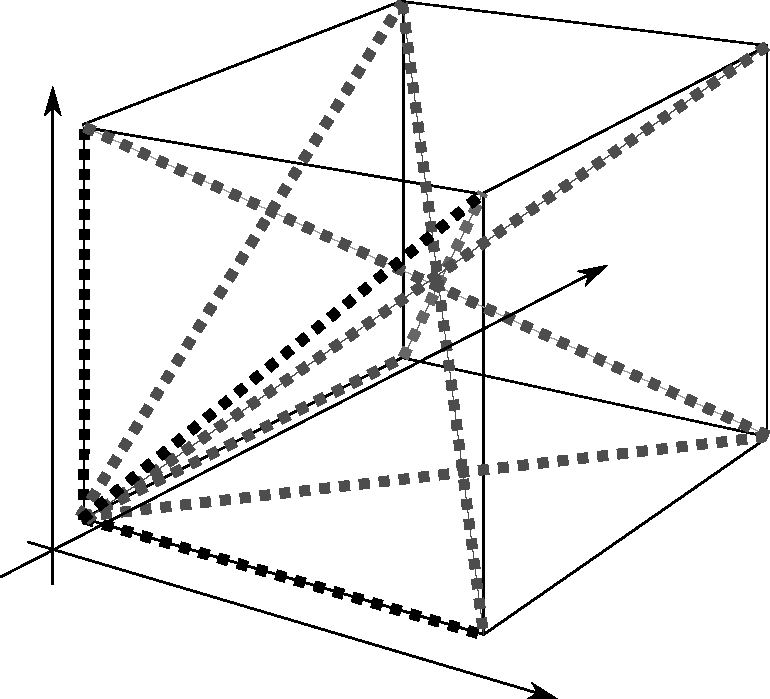
\includegraphics[width=0.25\textwidth]{sketches/collision-cube.pdf}
    \hspace{0.2cm}
    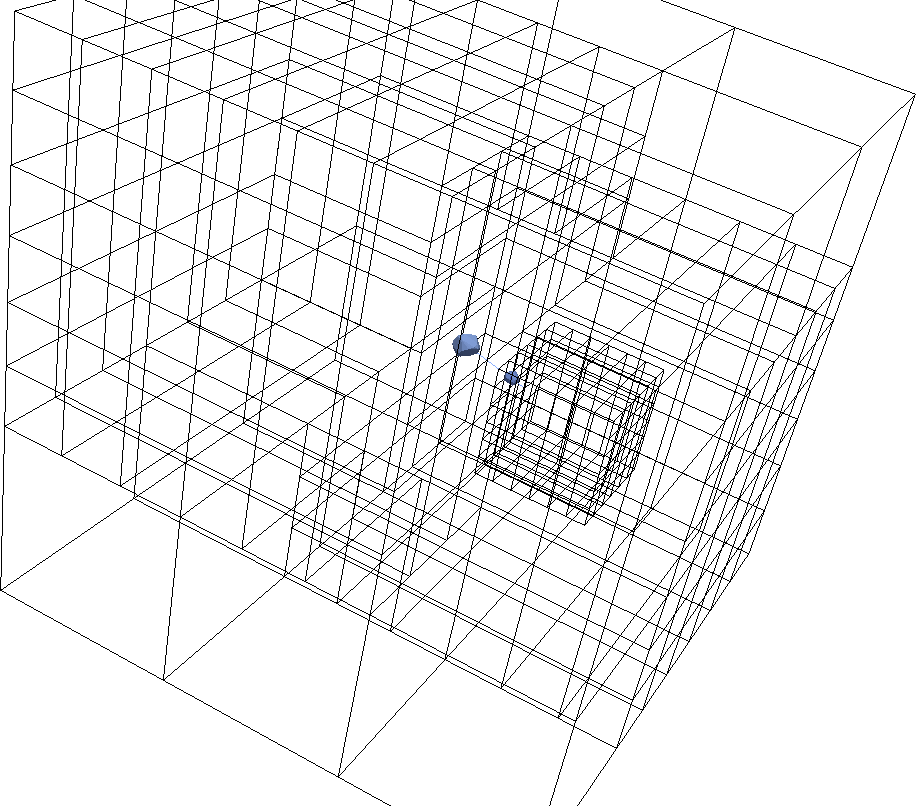
\includegraphics[width=0.3\textwidth]{experiments/two-bodies/visualisation/adaptive-grid01.png}
    \hspace{0.2cm}
    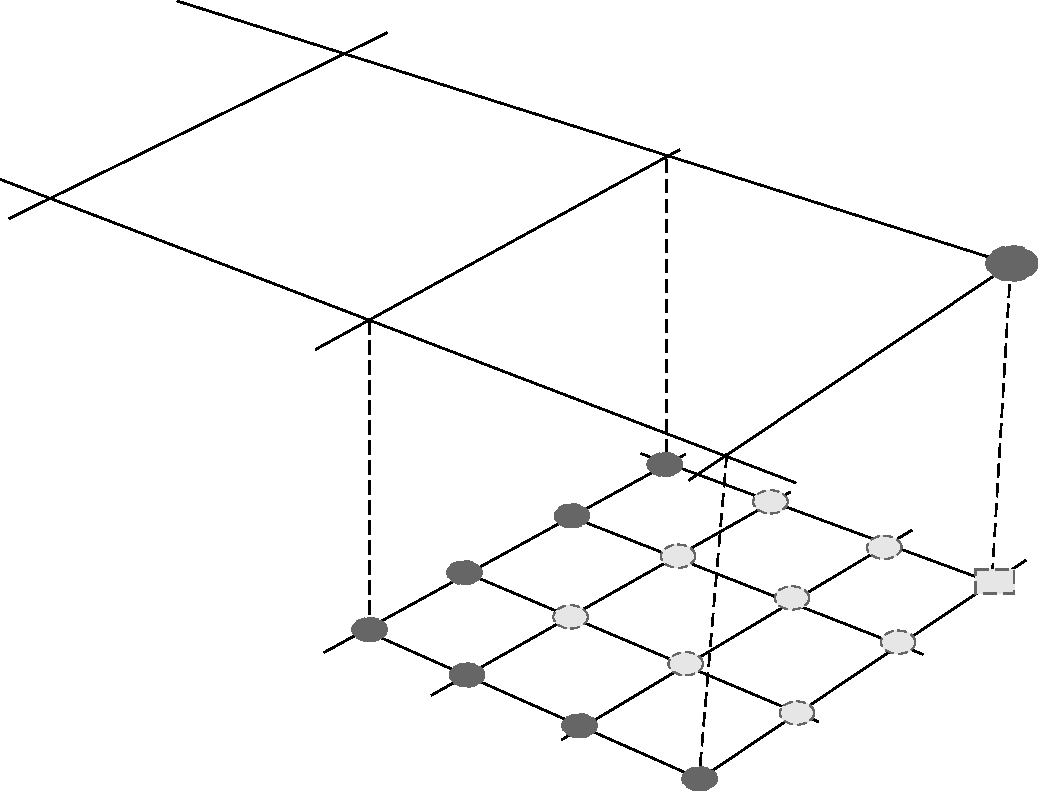
\includegraphics[width=0.3\textwidth]{sketches/multigrid.pdf}
  \end{center}
  \caption{
    Left: Whenever the grid traversal enters a cell, it checks whether particles
    assigned to one vertex do collide with particles assigned to another vertex.
    To avoid redundant collision computations, we check only some vertex pairs
    (dotted, larger lines).
    Middle: Two particles approach each other. As they are of different size,
    they might be held on different spacetree resolution levels.
    Right: In the adaptive case, particles are dropped from the coarse levels
    into the fine grid (rectangular marker) if new grid levels are added. The
    bright round vertices are children of the marked coarse grid vertex. The
    bright and the dark round markers' vertices together are the descendants of
    the marked coarse grid vertex.
  }
  \label{figure:collision-cube}
\end{figure}

We then write down the algorithm as a set of events, i.e.~we specify which
operations are performed if a vertex is read for the very first time \linebreak
(\texttt{touchVertexFirstTime}), if a cell is entered
(\texttt{enterCell}), and so forth.
Besides the actual grid hosting the particles, the grid sweeps build and
maintain two further sets of collision points (algorithm \ref{algorithm:grid-based-dem}).


\begin{algorithmic}[1]
  \Function{traverseGrid}{$\mathcal{C}$}
   \State $\mathcal{C}_{old} \gets \mathcal{C}$
   \State $\mathcal{C} \gets \emptyset$
   \While{traversal continues}
    \If{\texttt{touchVertexFirstTime}}
     \ForAll{particles $p$ associated to vertex}
      \ForAll{contact points $c \in \mathcal{C}_{old}$ associated to $p$}
       \State Update $f(p)$ through $c$
      \EndFor
      \State Update particle incl.~its triangles
     \EndFor
     \ForAll{particle pairs $(p_i,p_j)$ associated to vertex}
       \State $\mathcal{C} \gets \mathcal{C} \cup $
       \Call{findCollisions}{$p_i,p_j$}
     \EndFor
    \EndIf
    \If{\texttt{enterCell}}
     \ForAll{$2^d$ vertices adjacent to cell}
      \ForAll{particles $p$ associated to vertex}
       \If{particle should be associated to different vertex}
        \State Reassign particle
       \EndIf
      \EndFor
     \EndFor
     \ForAll{$(p_i,p_j)$ associated to different vertices (cmp.~figure)} 
      \State $\mathcal{C} \gets \mathcal{C} \cup $
       \Call{findCollisions}{$p_i,p_j$}
     \EndFor
    \EndIf
   \EndWhile
  \EndFunction

  %\Function{main}{$T$}   
  % \State $\mathcal{C} \gets \emptyset $
  % \State $t \gets 0 $
  % \For{$t < T$}
  %  \State \Call{traverseGrid}{$\mathcal{C}$}
  %  \State $t \gets t + \Delta t$
  % \EndFor
  %\EndFunction
  
 %\caption{A grid-based DEM implementation.}
 \label{algorithm:grid-based-dem}
\end{algorithmic}


Our grid-based realisation is characterised by few properties:
\begin{itemize}
  \item When we load a vertex for the very first time, we make all particles
  associated to this vertex move. 
  \item When we load a vertex, we do compare all the particles associated to
  this vertex with each other and identify collision points. The comparison of
  particles associated to different vertices is realised when we enter a cell.
  Here, we do compare the vertex pairs from Figure \ref{figure:collision-cube}---left bottom
  front vertex with right bottom front vertex, all diagonal combinations, and
  so forth---such that we avoid multiple evaluations of vertex pairs. For 
  boundary cells, some special case distinctions yielding additional checks are
  added. If a cell is traversed, we assume that all its adjacent vertices are
  available, i.e.~have been read before.
  \item Whenever we run into a cell, we run through all the adjacent vertices
  and their particles. They all already have an updated position, as any vertex
  has been loaded before and thus been subject to \texttt{touchVertexFirstTime}.
  If a particle is associated to the 'wrong' vertex as it has moved and should 
  be assigned to another vertex of the cell, we do the reassignment. A particle
  may move at most one cell of its corresponding level a time.
  \item The vertex comparisons yield a set of collision points. This set is kept
  persistent for the subsequent traversal: one time step of the scheme is
  realised per two grid traversal. The amortised cost however still is one time
  step per grid traversal. This scheme picks up the idea of pipelining
  \cite{Plimpton1995}. Collision data is mapped onto the particles when we read a
  particle for the first time in the subsequent traversal. Immediately after the
  forces acting on a particle are determined, we do update the particle's
  property and also update the geometric data due to translation and rotation.
\end{itemize}

\noindent
The extension of the present scheme to multiscale trees is detailed below.
To make the algorithm correct, each contact point set between two particles does
exist twice with inverse normals.
Each set furthermore is augmented with a copy of the corresponing partner
particles' global data (mass, velocity, momentum).
Otherwise, we would have to search for this data and build up global indices,
and have to be aware that the particle's data already might have been subject to
the next time step.


The algorithm realises a single-pass policy. Geometric data is written only once
per traversal, and is read only when we read in a vertex for the first time and
when we run through a cell.
The implementation's pressure on the memory subsystem thus is minimalistic as
long as the spatial and temporal grid access locality \cite{dime} is high which
yields high cache hit rates.
We rely on a space-filling curve to
run through the grid \cite{Weinzierl:2009:Diss,Weinzierl:11:Peano} and thus
guarantee such a two-fold locality.


\noindent
More sophisticated explicit schemes can be realised with the same single-touch
policy if we hold additional data per particle (acceleration, e.g.).
Such an approach picks up ideas of pipelining \cite{Plimpton1995}.


{\bf Regular grid.}
The spacetree formalism allows us to realise at least three grid variants. 
A very simple refines all spacetree nodes all the time as long as the resulting
cell mesh size is bigger than the largest particle diameter.
Such a strategy yields a regular Cartesian grid. 

{\bf Dynamically adaptive grid.}
Our dynamically adaptive grid is characterised by two ingredients: mesh
refinement control and inter-grid particle treatment.
In \texttt{touchVertexFirstTime}, our code analyses what the smallest diameter
of all the particles held by the vertex is.
If this diameter is smaller than $1/3$ of the mesh width corresponding to the
vertex's level, then the region around the vertex is refined.
If we run into a vertex, we check whether there are any spatially coinciding
vertices in the tree on a coarser level.
If such vertices do exist, we run through all of their particles and move them
one level down if the diameter permits.
The scheme successively drops the particles down the grid hierarchies.

\begin{figure}
 \begin{center}
  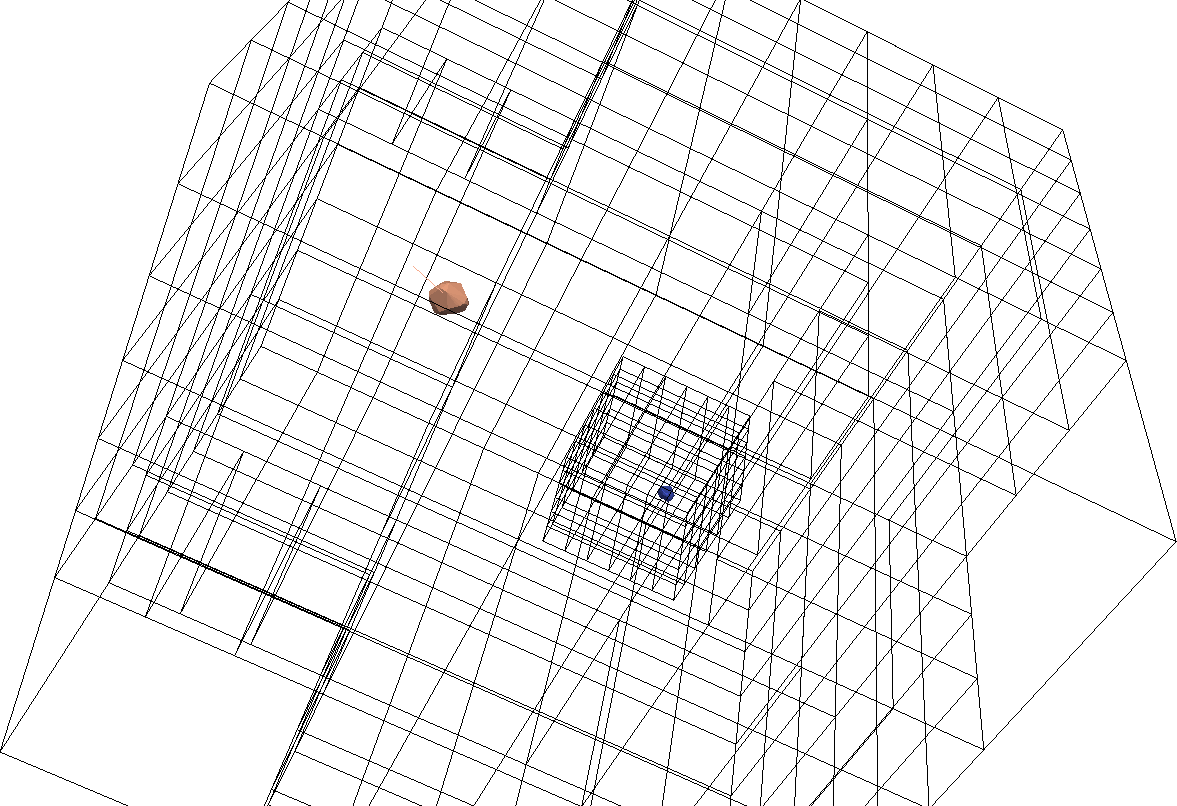
\includegraphics[width=0.4\textwidth]{experiments/two-bodies/visualisation/adaptive-grid00.png}
  \hspace{1.1cm}
  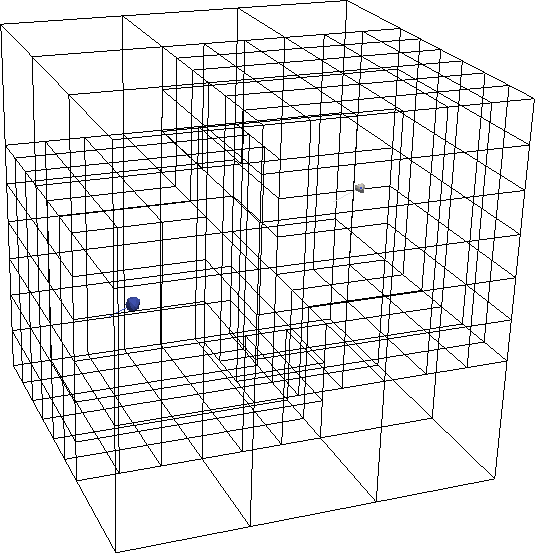
\includegraphics[width=0.25\textwidth]{experiments/two-bodies/visualisation/reluctant-adaptive-grid00.png}
  \\
  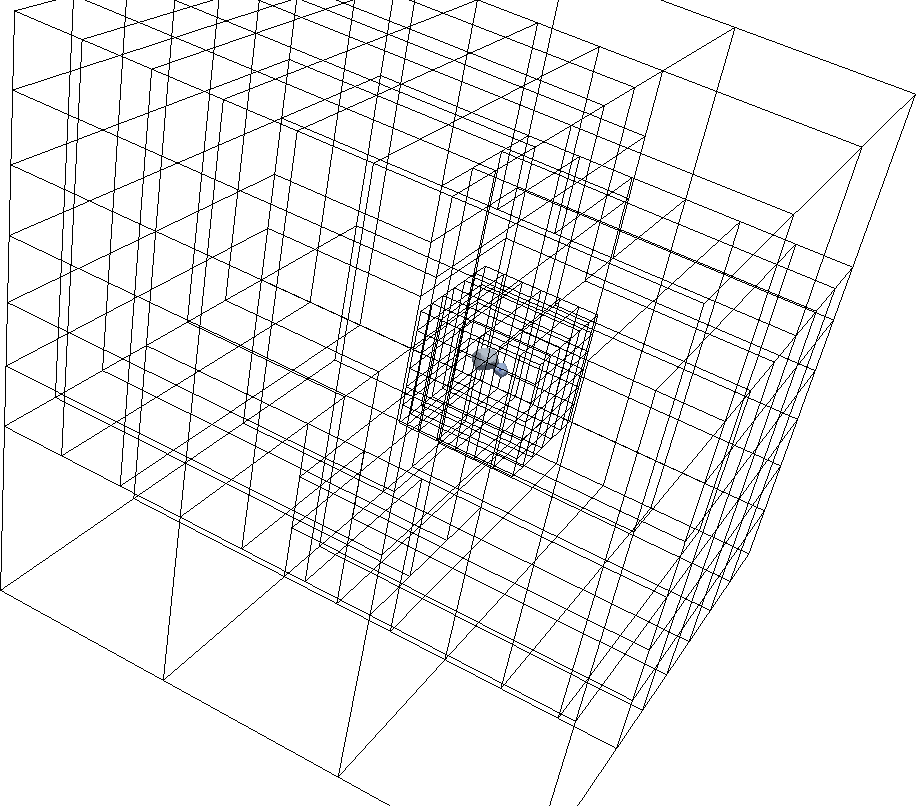
\includegraphics[width=0.3\textwidth]{experiments/two-bodies/visualisation/adaptive-grid02.png}
  \hspace{1.1cm}
  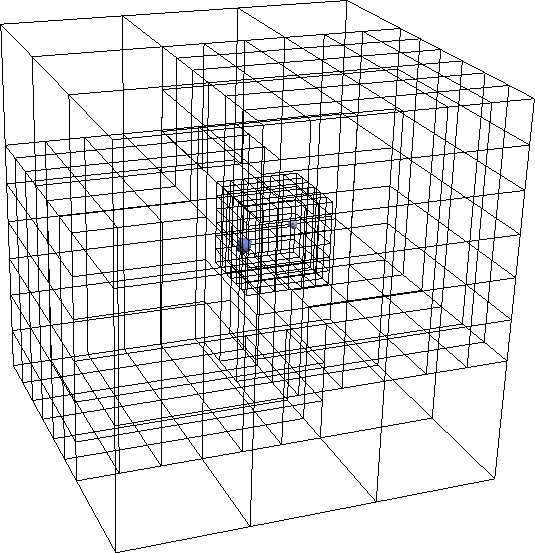
\includegraphics[width=0.3\textwidth]{experiments/two-bodies/visualisation/reluctant-adaptive-grid02.png}
% 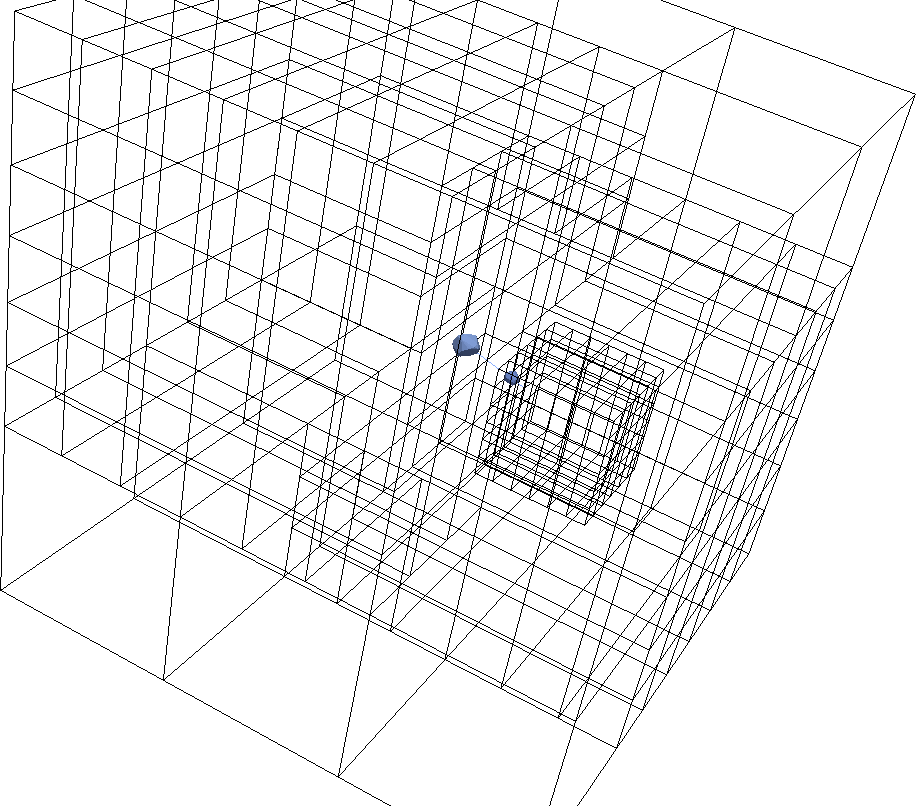
\includegraphics[width=0.3\textwidth]{experiments/two-bodies/visualisation/adaptive-grid01.png}
%   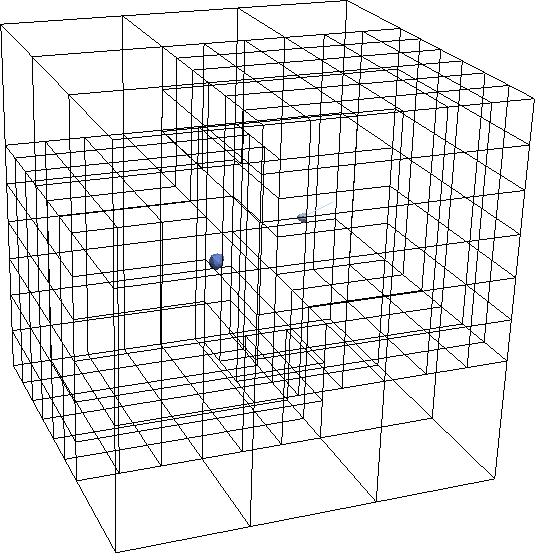
\includegraphics[width=0.3\textwidth]{experiments/two-bodies/visualisation/reluctant-adaptive-grid01.png}\\
%   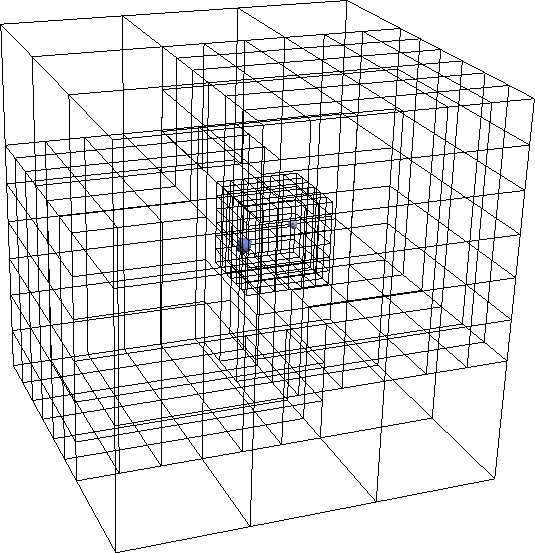
\includegraphics[width=0.3\textwidth]{experiments/two-bodies/visualisation/reluctant-adaptive-grid02.png}
%   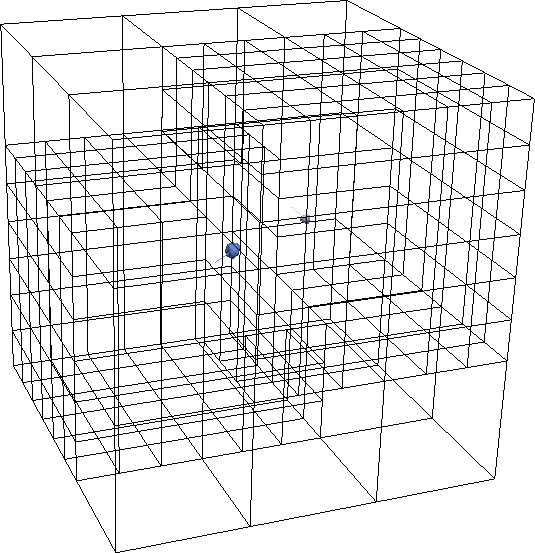
\includegraphics[width=0.3\textwidth]{experiments/two-bodies/visualisation/reluctant-adaptive-grid03.png}\\
 \end{center}
 \caption{
   Two particles crash into each other.
   The adaptive grid refining around each particle while its diameter
   constrains the mesh size (left column).
   The reluctant adaptive grid works with a coarser resolution as long
   as particles are far away from each other (right column).
   Just before they collide, the grid is refined and particles are dropped down
   the resolution levels.
 }
 \label{figure:adaptive-vs-reluctant-grid}
\end{figure}

We define two multiscale relationships between vertices (Figure
\ref{figure:collision-cube}).
A vertex $a$ is a child of a vertex $b$ if all adjacent cells of $a$ are
children of adjacent cells of $b$. $b$ is the parent vertex of $a$.
A vertex $a$ is a descendant of $b$ if at least one adjacent cell of $a$ is a
child of an adjacent cell of $b$. $b$ is an ancestor of $a$.
If we delete a vertex $a$ that holds particles, its particles are moved to the
next coarser level and assigned there to the nearest parent of $a$.
Each vertex holds a boolean marker that is set $\bot $ before the vertex is
read for the first time.
If a vertex holds a particle, all the markers of the vertices where it is a
descendent from are set to $\top$.
If a vertex whose adjacent cells all are refined holds $\bot$ at the end of the
multiscale traversal, we coarsen these refined adjacent cells.
We rely on a top-down tree traversal.
The refinement/coarsening procedure then can be evaluated on-the-fly.
It equals an analysed tree grammar \cite{Knuth71}.

For the multiscale contact detection, we extend the list of particles associated
to a vertex. 
There is the list of actually held particles and a list of virtual particles. 
We run through the grid top down, i.e.~a vertex always is read for the first
time before any of its descendants, and clear virtual particle list first.
Then, we add all particles held in the particle or the virtual particle lists of
any ancestor to the local virtual list.
If we compare all particles with each other that are held by the same vertex, we
do compare the actual particles with all other real particles as well as all
virtual particles.

{\bf A reluctant adaptive grid.}
The dynamically adaptive grid refines rather aggressive: Particles are always
dropped to their corresponing refinement level immediately. 
Fine grid regions thus follow 'their' particles (Figure
\ref{figure:adaptive-vs-reluctant-grid}).
This might introduce finer grids than actually required for contact detection
which is an overhead.
Given the one-cell-per-time-step constraint on the particle velocity, we also
restrict the maximum velocity or time step rigorously.
For the present work, this does not have a major impact as we apply uniform
small time step sizes globally. 
For schemes with local time stepping, it however is important, besides overhead
discussions, to keep the grid as coarse as possible as this facilitates big
time step sizes.

Our reluctant adaptive grid works with coarser adaptive grids than the plain
variant through two modifications of the refinement procedure: 
On the one hand, we refine the region around a vertex if the previous criterion
holds and the vertex holds at least two particles.
If only one particle is holds, we stick locally to the grid no matter what the
particular diameter is.
Throughout the inter-vertex contact detection in \texttt{enterCell}, we further
bookkeep the minimum diameter of all the particles involved. 
If this minimal diameter is smaller than the cell, we do refine this cell, too.

\subsubsection{Vectorization}

There are three different types of data sets in our minimalistic DEM codes: 
geometric data, behavioural data and meta data. 
Behavioural data is collision data.
It is modelled as struct with location and a normal vector.
Sets $\mathbb{C}$ of collision points are modelled as (dynamic) array of structs
(AoS) augmented with a copy of the collision partner as detailed before.
Spacetrees are our meta data.
The geometry data finally determines how straightforward and fast the collision
detection is. Collision detection is the computationally heavy activity in the
algorithm.
While other DEM discussions speak of a computational phase \cite{Wachs2012, Wachs2012a, Rycroft2012, Parteli2013}, we
prefer the term activity, as the collision detections are split among the grid traversal
and interwoven with other activities.

\begin{figure}
 \begin{center}
  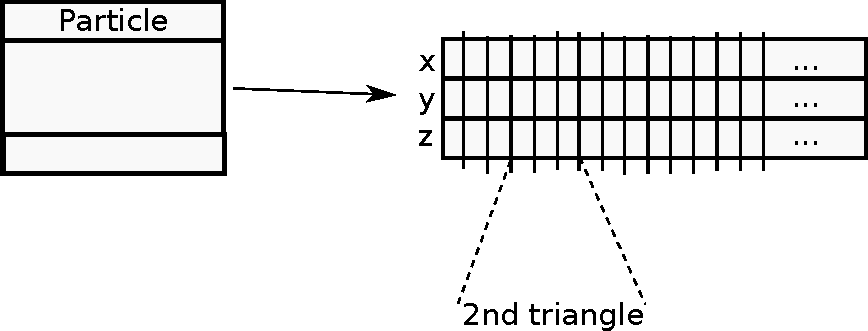
\includegraphics[width=0.5\textwidth]{sketches/data-structure.pdf}
 \end{center}
 \caption{
   Right: The two layer data layout of our DEM code with an AoS on the particle
   level but SoA for the vector entries with replicated vector entries.
 }
 \label{figure:data-structure}
\end{figure}

We propose to realise the geometric data in two layers (Figure
\ref{figure:data-structure}).
A hull struct holds all particle properties such as velocities, rotation, mass,
geometric centre and mass centre.
Vertices refer to these hulls with arrays of structures (AoS).
Hulls link with pointers to the actual geometric data. 
This data is realised as structure of array, i.e.~there is a sequence of
x-coordinates, a sequence of y-coordinates and a sequence of z-coordinates.
These sequences are blown up with redundant data.
The first three entries in the x array hold the x coordinates of the three
vertices of the first triangle of the particle mesh.
The entries four through six hold the coordinates of the second triangle and so
forth. 
The degree of redundancy is determined by the particle mesh.

We accept the increased memory consumption of such a structure but in return are
able to avoid any indirect addressing, process all geometry data in the
collision checks in a stream-like fashion and can align all vector entries. 
SoA data are notouriously difficult to handle if subsets of a dataset are to be
transferred or data is to be reordered \cite{Eichenberger2004}.
In our particle handling, a particle is an atomic unity.
It is never teared apart or resorted during the simulation run.
A particle mesh is topologically invariant.


\begin{figure}[!h]
\centering
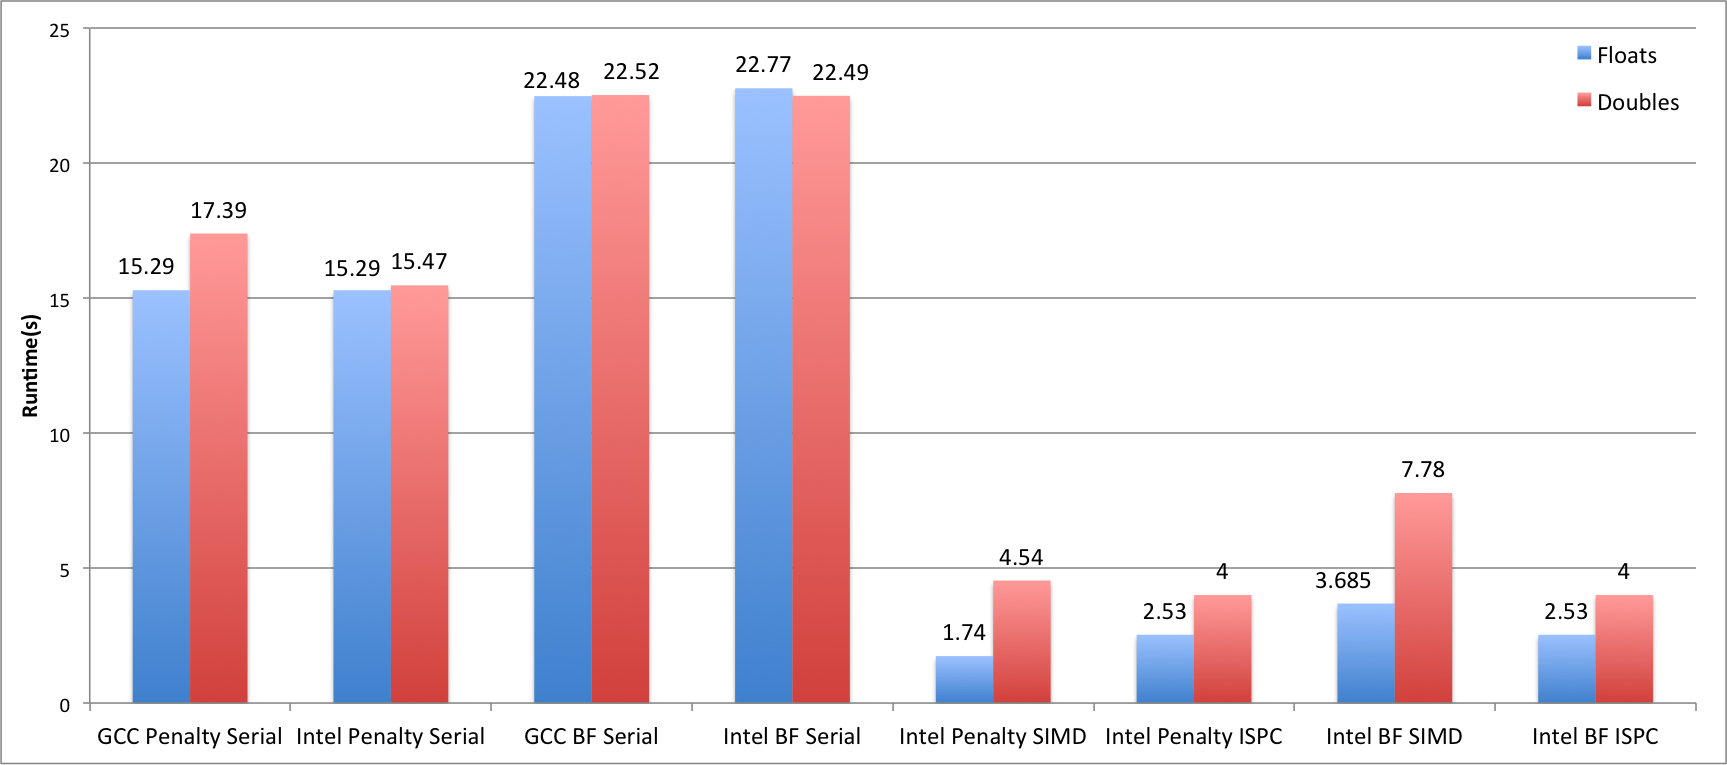
\includegraphics[width=1\textwidth]{perf} \protect\caption{\label{fig17}Run-time comparison of the sequential and parallel penalty and brute force methods using float and double precision, using ISPC, Intel, GCC compilers on a single AVX2 core, ten million pairs of triangles.}
\end{figure} 

In Figure \ref{fig17} SIMD implementations are compared against serials. For brute force, serial Intel and GCC are the slowest with no significant difference in using either precision this is due to lower arithmetic intensity. Intel SIMD  brute force shows 6x speedup compared to its serial sequential variant using single precision. Speed up in double precision is lower(~3x times), both experiments reflect the effect of branching involved in brute force. 
The penalty method reaches 4x speed up for double precision and 8x speedup for single precision. This makes it the fastest algorithm. Intel serial code is significantly faster than Intel and GCC versions of Brute force. GCC compilers for serial are slightly slower, but still faster than brute force GCC serial. The ISPC compiler for brute force is capable to do vectorization bette for double precision than the Intel compiler. As wer haven't studied the resulting assembler code we cannot identify where the difference between ISPC and C come from. All performance tests (Figure \ref{fig17}) use AVX2 (Advanced Vector Extensions) instruction set on an Intel Sandy Bridge 2.0GHz i5 CPU with a memory of 600 MHz DDR3 RAM.

\begin{table}[h]
\begin{center}
    \begin{tabular}{ | l | l | l | p{5cm} |}
    \hline
\multicolumn{3}{ |c| }{Intel C++ Compiler Serial Double Precision} \\
\hline
    Algorithm & Penalty Method & Brute Force Method\\ \hline
    Runtime unhalted (s) & 15.47 & 22.49  \\ \hline
    MFLOPS/s & 1073 & 962  \\ \hline
    CPI & 0.49 & 0.48 \\ \hline
    Memory BW M/s & 579 & 408 \\ \hline
    Data Volumn GB & 6.7 & 6.77 \\ \hline
    \end{tabular}
    \caption{64bit sequential computation; solving ten million random triangle pairs using the two methods.}
    \label{table1}
\end{center}
\end{table}

In Table \ref{table1} using likwid [49] both methods are not memory (Memory BW Bandwidth Megabyte per second) but compute-bound. For the machine used, the maximum memory throughput is 13 GB/s, so memory bandwidth does not peak. The data volume is same for both methods as input and output is identical. 

\begin{table}[h]
\begin{center}
    \begin{tabular}{ | l | l | l | p{5cm} |}
    \hline
\multicolumn{3}{ |c| }{Intel C++ Compiler SIMD Double Precision} \\
\hline
    Algorithm & Penalty Method & Brute Force Method\\ \hline
    Runtime unhalted (s) & 4.54 & 7.78  \\ \hline
    MFLOPS/s & 3202 & 2808  \\ \hline
    CPI & 1.26 & 0.91 \\ \hline
    Memory BW M/s & 1424 & 902 \\ \hline
    Data Volumn GB & 5.15 & 5.2 \\ \hline
    \end{tabular}
    \caption{64bit SIMD computation; solving ten million random triangle pairs using the two methods.}
    \label{table2}
\end{center} 
\end{table}

In Table \ref{table2} the SIMD implementation for both methods increase pay off significantly. Compared to serial counterparts both achieve at least 2x times speedup, with penalty achieving  3.40x speedup, and brute force 2.89x speedup. The theoretical maximum speedup that is possible to achieve is 4x times for 64bit precision 256bit wide register. ISPC compilers however as shown in Figure \ref{fig17} double precision give 4x speedup. For 32bit precision the speedup is near 8x (figure \ref{fig17}).

\subsubsection{Shared Memory}

We introduce three levels of shared memory parallelisation on a single machine that exploit multiple levels of locality. The hierarchical categorisation of the methods is based upon the abstract algorithmic distance between shared resource parallel utilisation and actual arithmetic computation. At the highest level we exploit  data access independence of vertex touches we assign cell block tasks to threads. Within each vertex touch particle pairs are grouped into aligned memory blocks thus tasks are launched between particle-to-particle comparisons. Lastly within each particle pair at the innermost level tessellation elements of the mesh are dichotomised and parallel locality is held for the underlying vectorized contact solver.

Three levels of multicore parallelisation:\\

a) cell level cell-to-cell thread units\\

b) cell vertex level particle-to-particle thread units\\

c) particle level mesh-to-mesh thread units\\

Respectively, we have three parameters to decompose the simulation domain. $Rmin$, $Rmax$ parameter for max and min radius of particles, $m$ for mesh density, $p$ for number of particles in the domain. These allow observation of the interplay between performance and particle geometry and dynamics within a grid in a modern NUMA architecture. For scaling measuring we use the hybrid and the brute force solvers.

%Initial-termination conditions
For the experiment the initial space configuration of the particles in respect to the grid is homogeneous and aligned per cell. Initial conditions for the particle dynamics are governed by only gravity and termination is defined by the number of iteration that the granulates are rest condition with energy dissipated on the ground. Termination phase is known a priori. We utilise regular grid and reluctant-adaptive grids for space decomposition and and grid adaptivity to granular kinematics. 

\iffalse
\begin{figure}[htb]
	\centering
	\begin{subfigure}{0.5\textwidth}
  		\centering
    	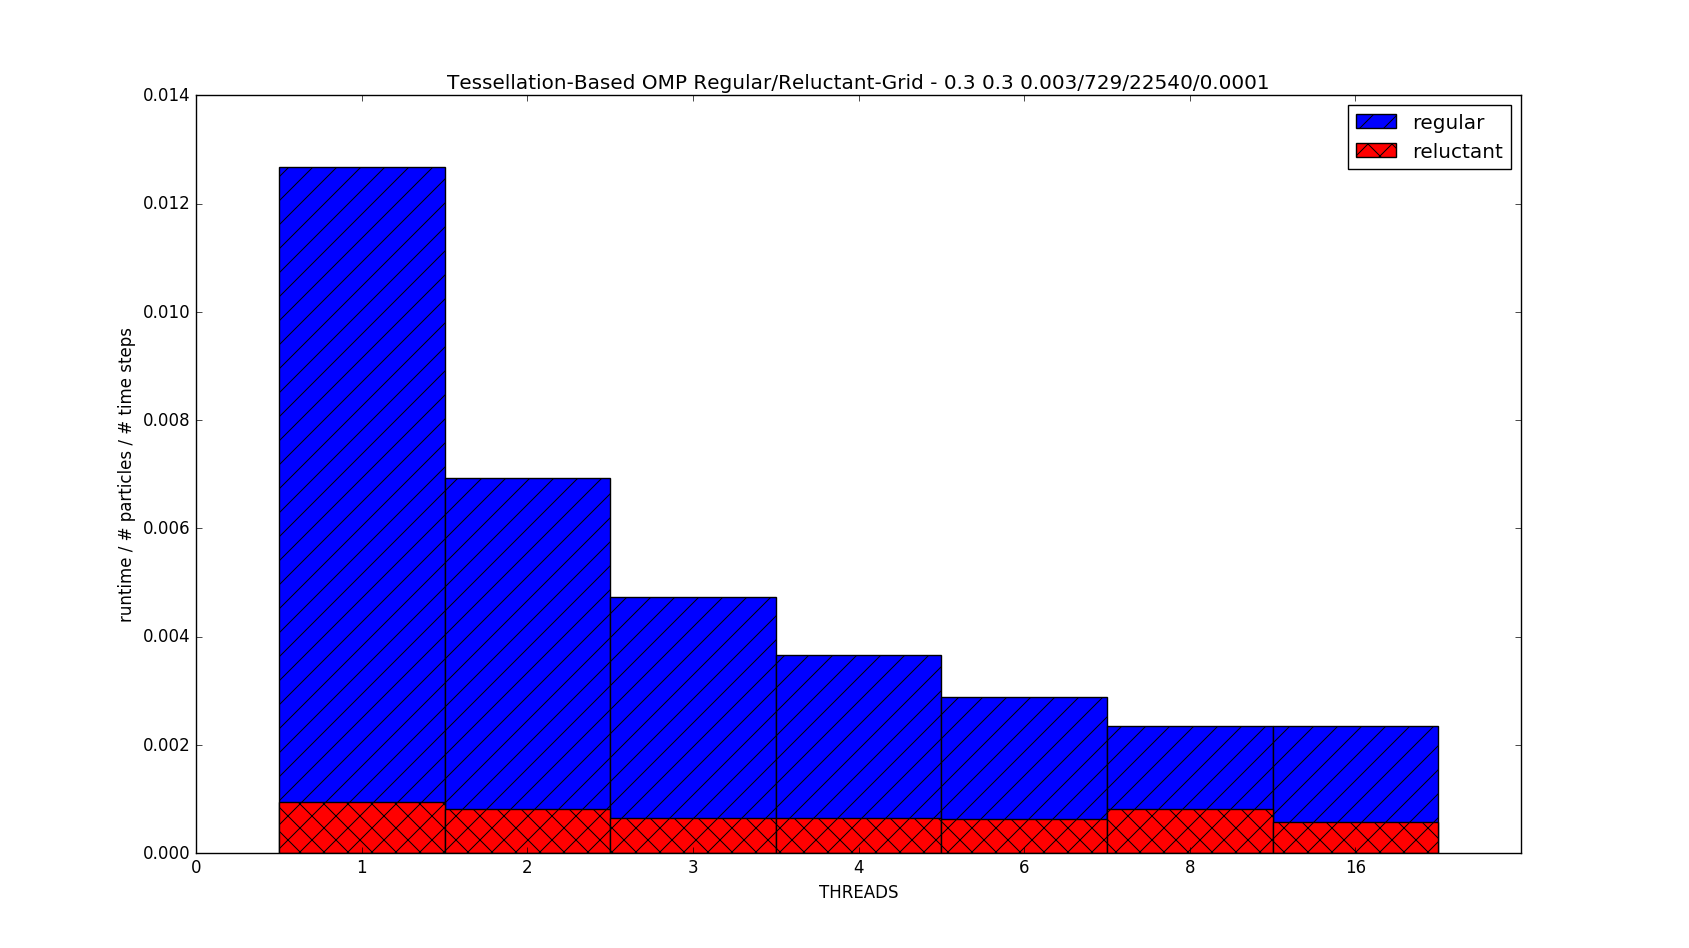
\includegraphics[width=1\textwidth]{experiments/omp/omp_mesh_regular-reluctant_20.png}
  		\caption{Shared memory scaling 22540 elements.}
  		\label{figure:omp_regular_reluctant_triangle_200}
	\end{subfigure}%
	\begin{subfigure}{0.5\textwidth}
  		\centering
    	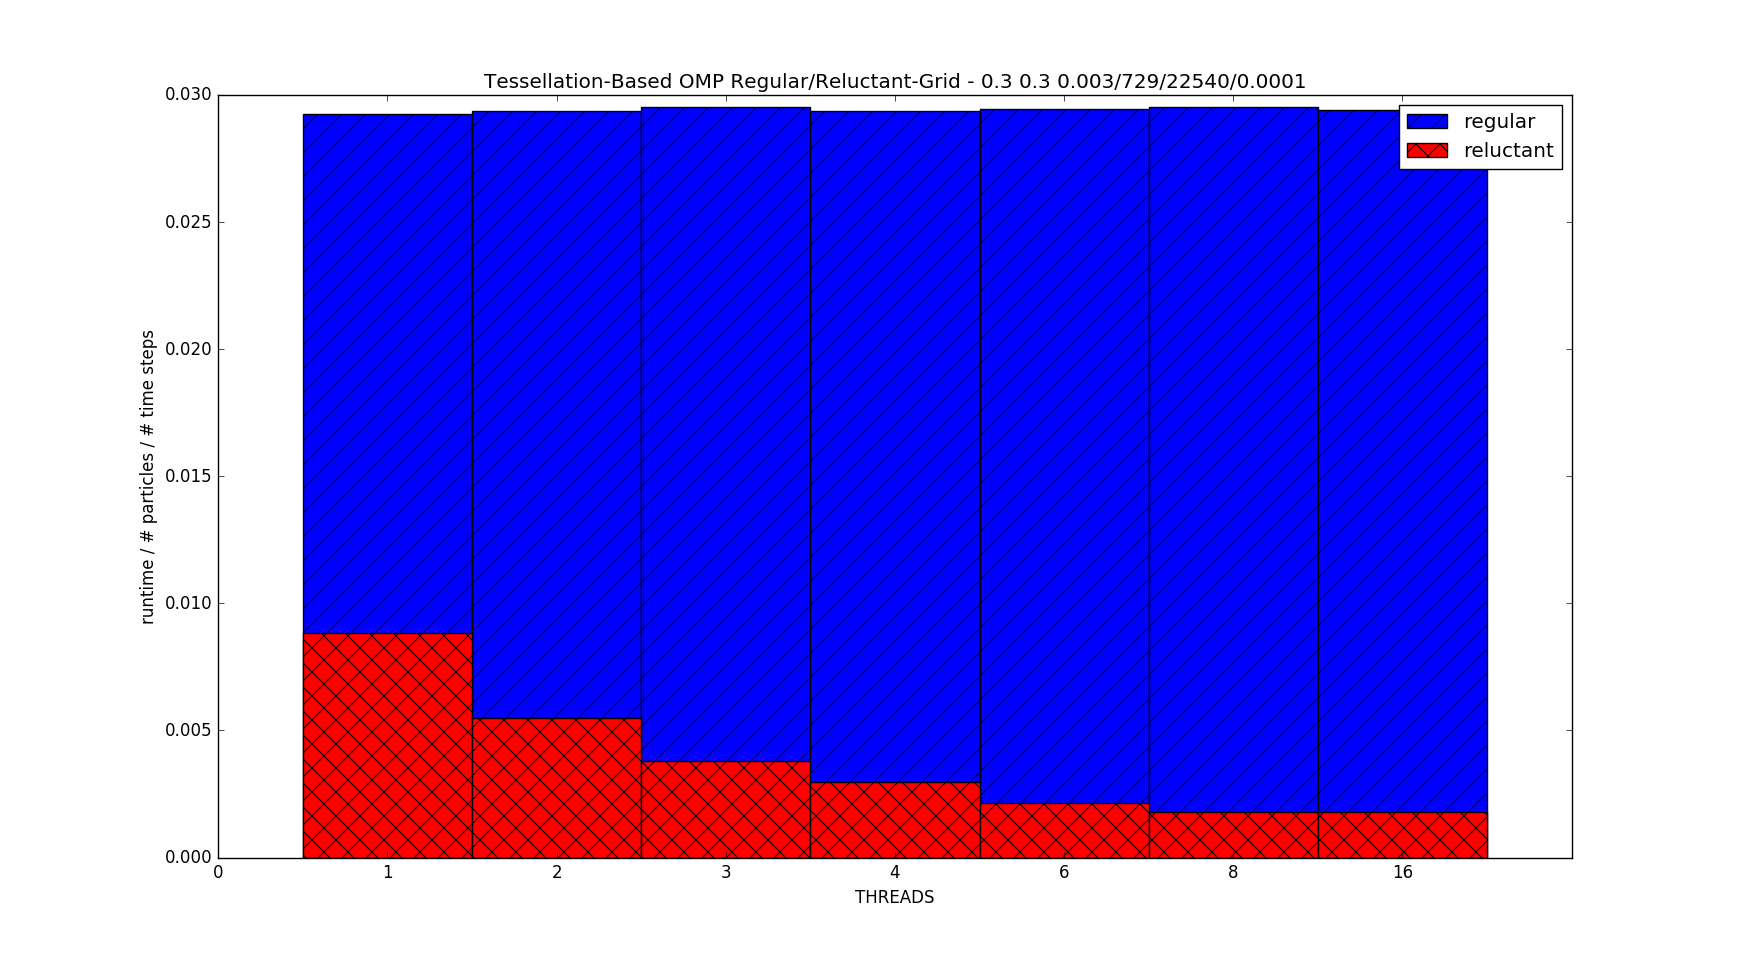
\includegraphics[width=1\textwidth]{experiments/omp/omp_mesh_regular-reluctant_200.png}
  		\caption{Shared memory scaling 98540  elements.}	
  		\label{figure:omp_regular_reluctant_triangle_200}
	\end{subfigure}
\end{figure}
\fi

\begin{figure}[htb]
  \begin{center}
    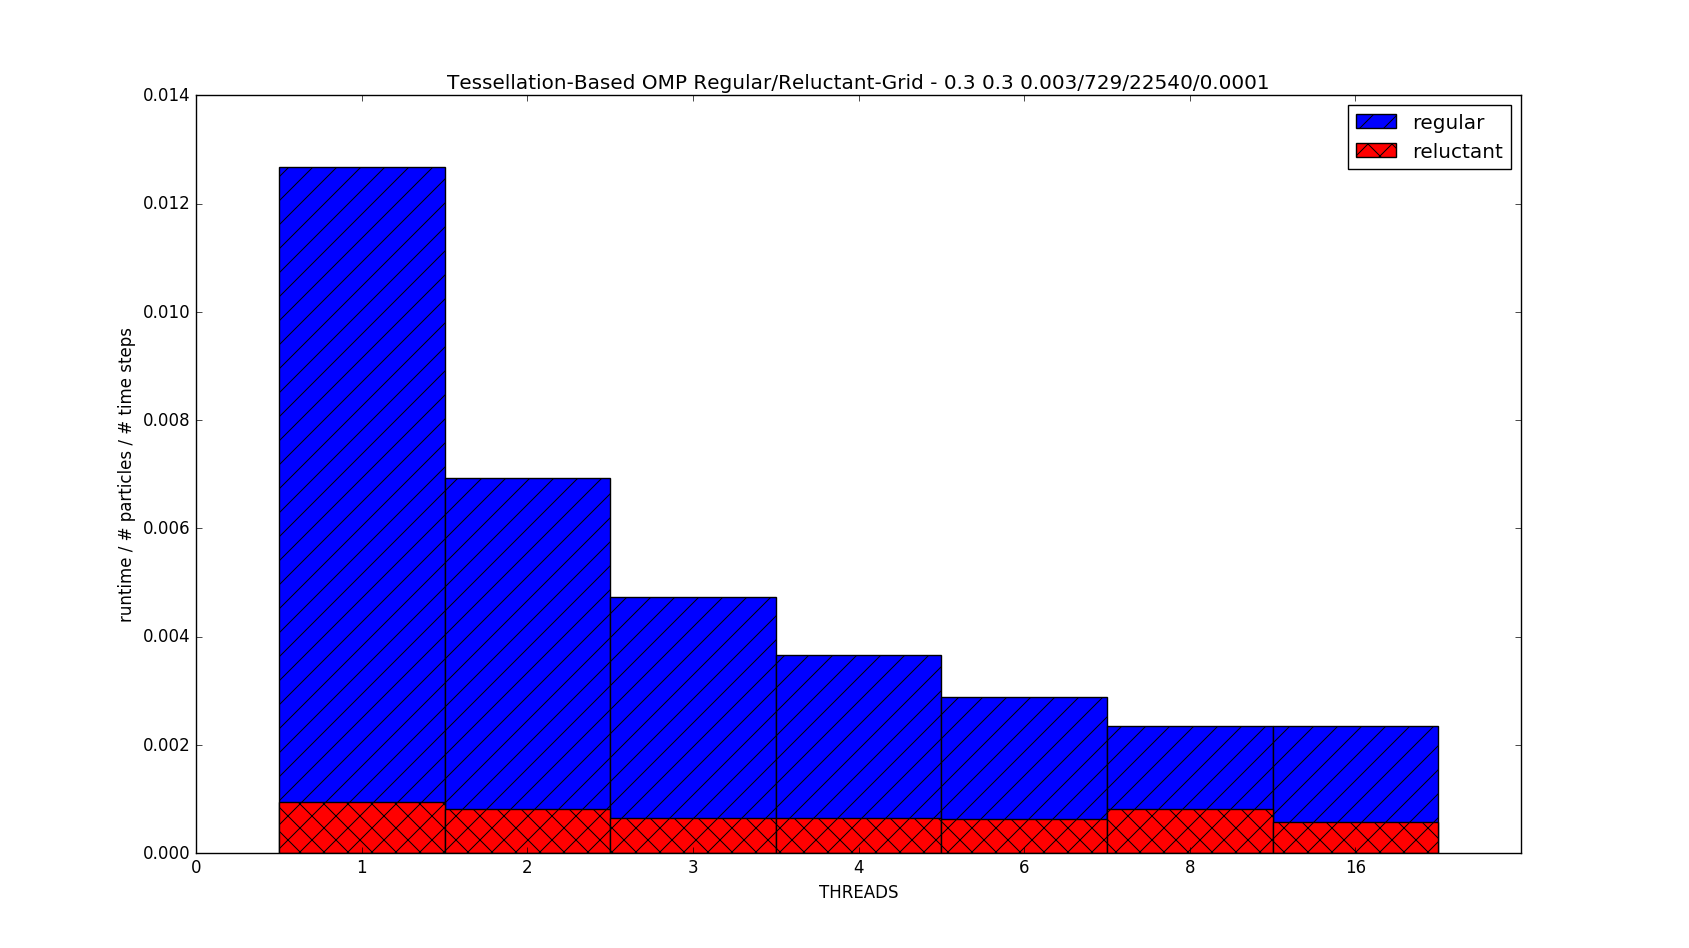
\includegraphics[width=0.7\textwidth]{experiments/omp/omp_mesh_regular-reluctant_20.png}
  \end{center}
  \caption{Grids shared memory scaling 22540 triangle elements (BF solver).}
  \label{figure:omp_regular_reluctant_triangle_20}
\end{figure}

\begin{figure}[htb]
  \begin{center}
    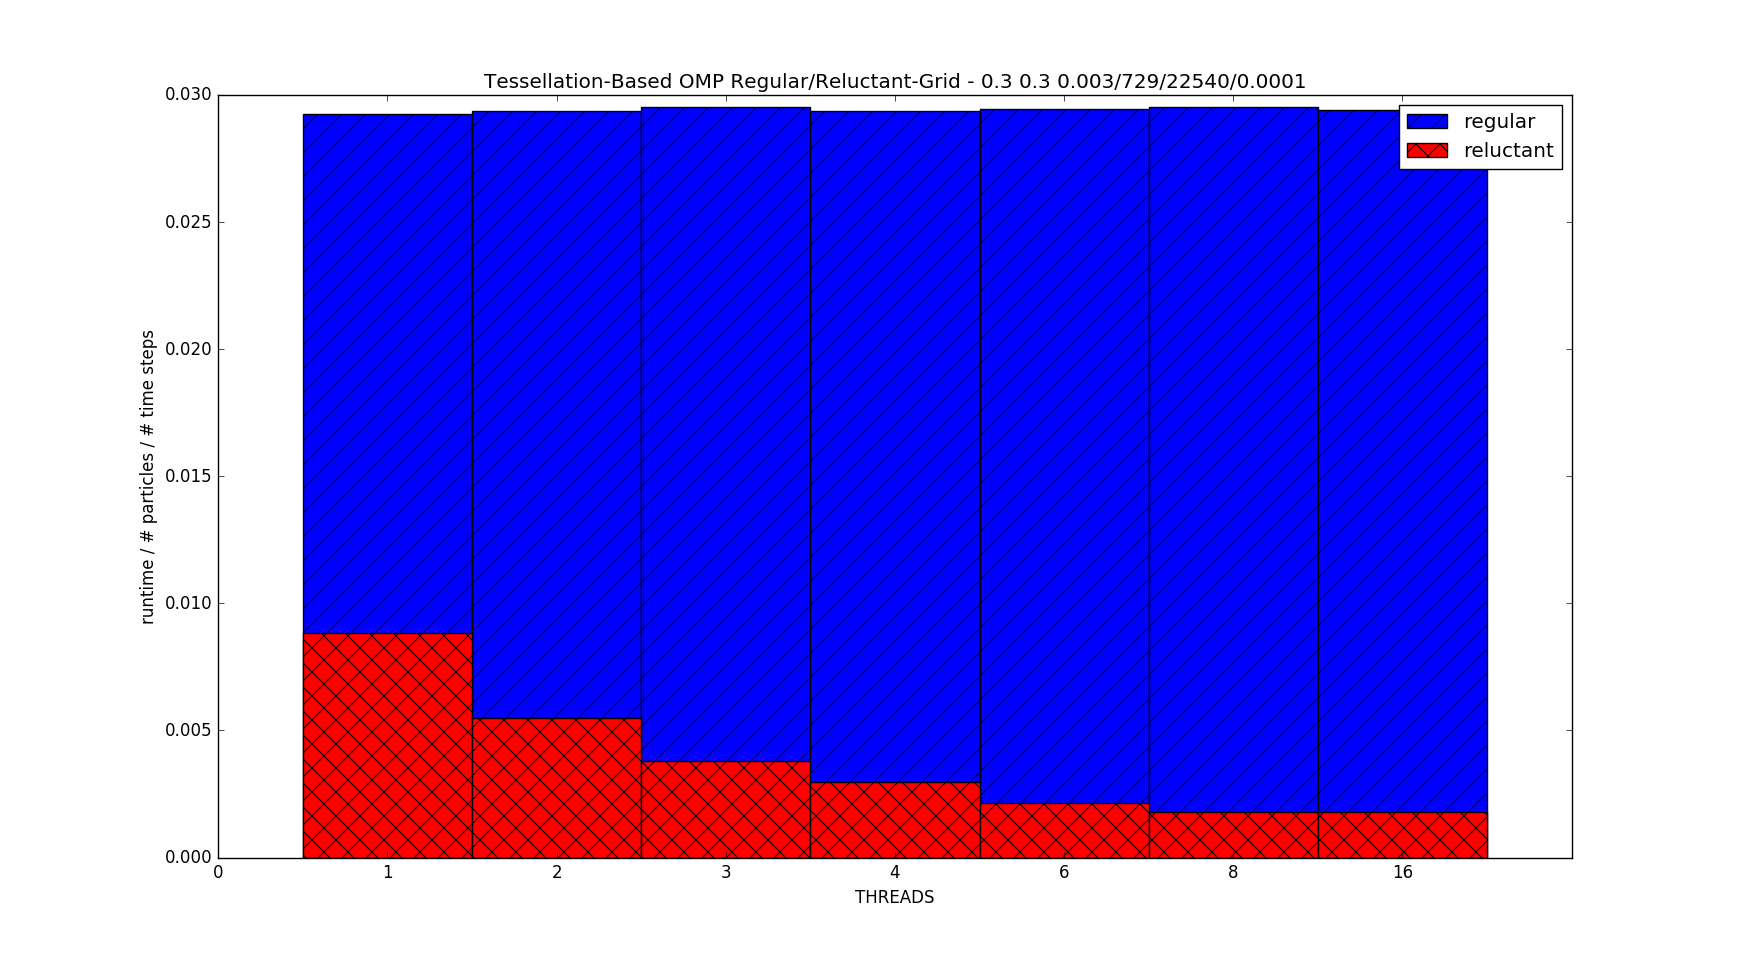
\includegraphics[width=0.7\textwidth]{experiments/omp/omp_mesh_regular-reluctant_200.png}
  \end{center}
  \caption{Grids shared memory scaling 98540 triangle elements (BF solver).}
  \label{figure:omp_regular_reluctant_triangle_200}
\end{figure}


%STEP A
Beginning at the innermost tessellation-level with a regular grid (figure \ref{omp_regular_reluctant_triangle_20}) on a NUMA ivy bridge system the code scales linearly up to the eight-core single die. As the size of the problem increase for weak scaling (figure \ref{omp_regular_reluctant_triangle_200}) the computation to memory bandwidth rate ratio is no longer sustainable computation to scale over multiple cores. Similarly on a small computational domain (figure \ref{omp_regular_reluctant_triangle_20}, blue) with minimum weighted threads grid adaptivity doesn't pay off as thread initialisation, scheduling, grid adaptivity and memory access overhead dominates over arithmetic intensity. Contrary to regular grid, adaptivity allows up-scaling towards both increasingly larger computations (figure \ref{omp_regular_reluctant_triangle_200}) and number of cores as long as bandwidth, compute bounds are not reached or thread overheads are not the bottleneck. In all cases the brute force solver does not scale pass the second die interconnect as communication to memory stagnates.

\begin{figure}[htb]
  \begin{center}
    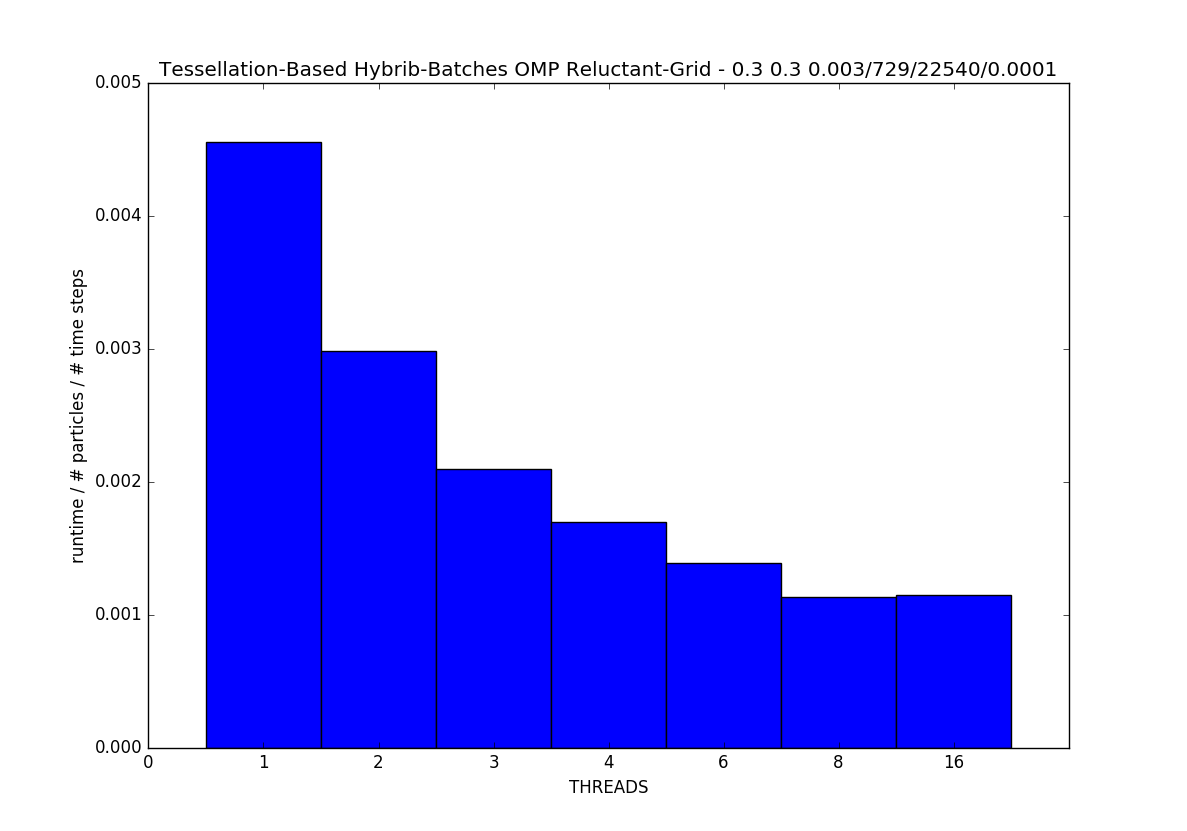
\includegraphics[width=0.7\textwidth]{experiments/omp/hbatches_omp_triangles_200.png}
  \end{center}
  \caption{Triangle based shared memory running hybrid-on-batches (HBatches).}
  \label{figure:hbatches_triangles_triangle_omp}
\end{figure}

Arithmetic, bandwidth intensity and data access patterns vary among solvers in the innermost level and can yield different performance results. The hybrid solver is parallelised in two different hybrid schemes triangle-to-triangle pairs and triangle-to-triangle batches, both launch different types of threads. For the hybrid-on-batches solver the tessellation-based threads
are $n$ triangle batches wide while hybrid-on-triangles solver relies on fine couples of threads. The non-deterministic nature and error-prone distribution of triangles of the hybrid algorithm as discussed in Chapter {-hybrid chapter-} would suggest that alternative scheduling would pay off. But for our experiments dynamic and guided thread scheduling don't have a performance gain but they rather create scheduling overhead due to error distribution in triangle pairs and due to the granularity of our batches. For the hybrid-on-triangles that is also the case because although the arithmetic intensity is dense in the solver, it doesn't last long enough to significantly overlap the cost of threading overhead. 

\begin{figure}[htb]
  \begin{center}
    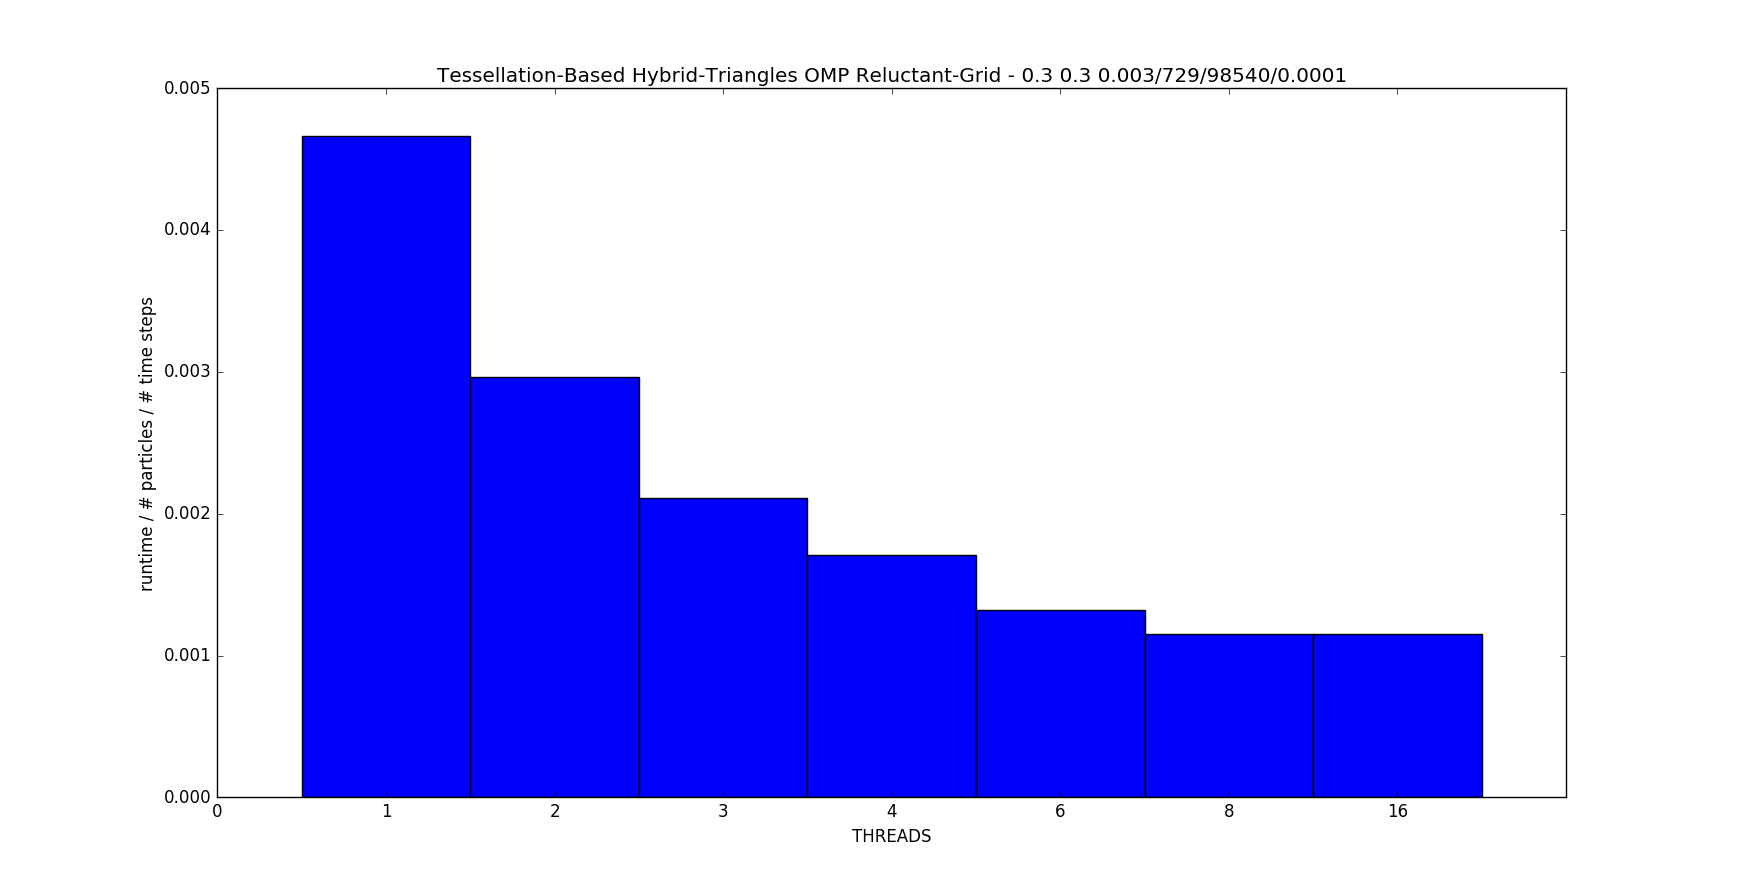
\includegraphics[width=0.7\textwidth]{experiments/omp/htriangle_omp_triangles_200.png}
  \end{center}
  \caption{Triangle based shared memory running hybrid-on-triangle-pairs (HTriangles)}
  \label{figure:htriangles_triangles_triangle_omp}
\end{figure}


\begin{figure}[htb]
  \begin{center}
    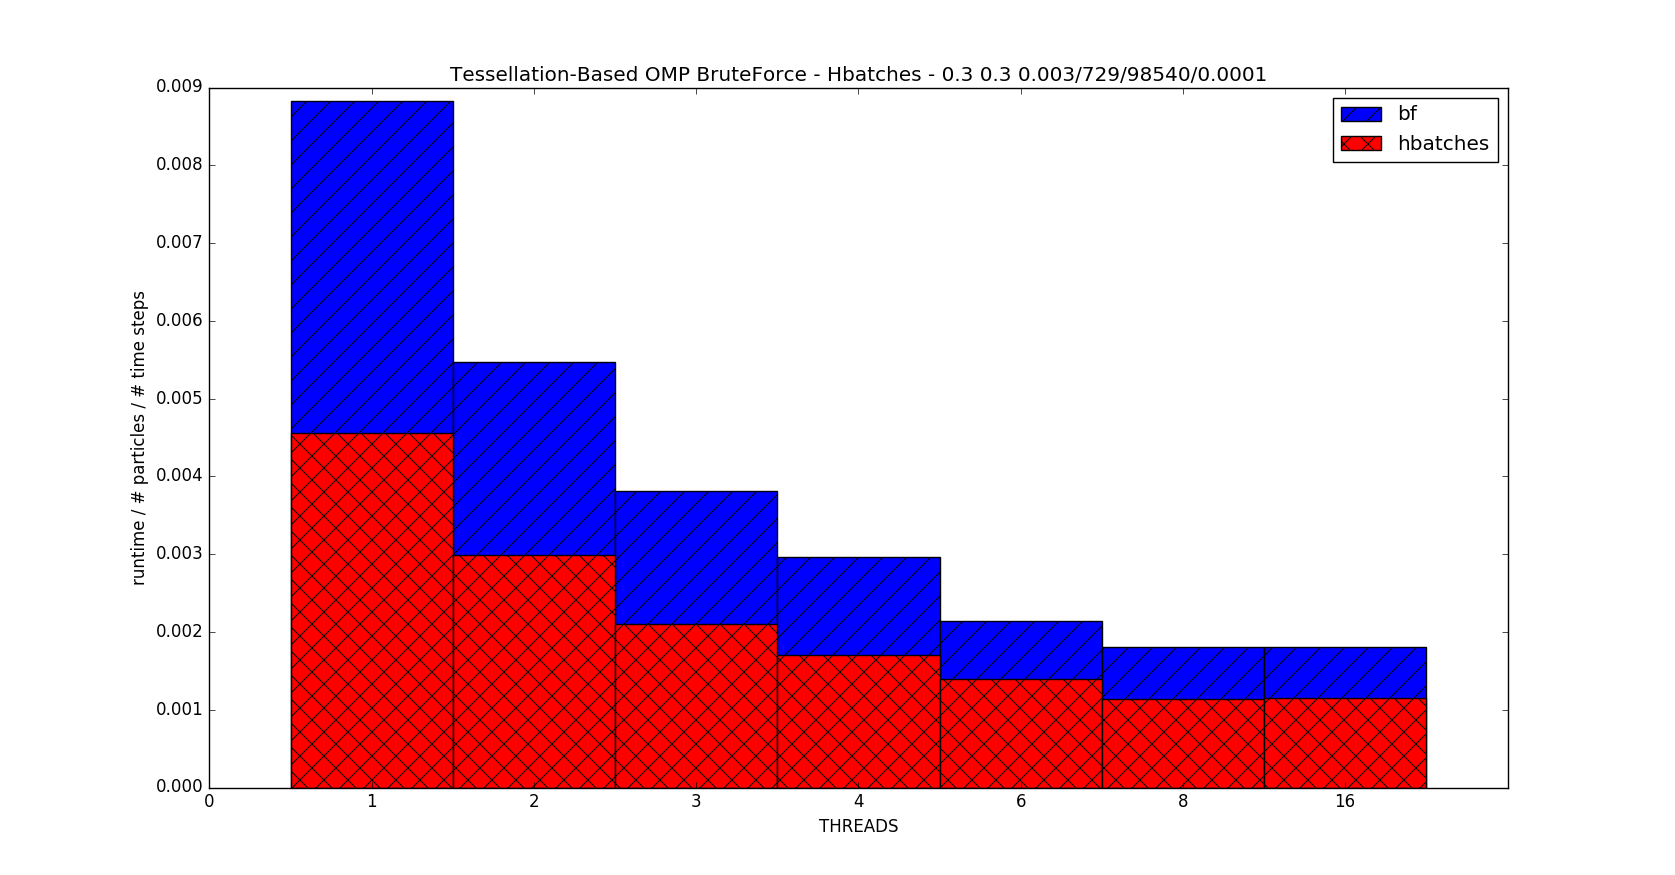
\includegraphics[width=0.7\textwidth]{experiments/omp/bf_vs_hbatches_omp_200.png}
  \end{center}
  \caption{Triangle based shared memory running hybrid-on-triangle-pairs (HTriangles)}
  \label{figure:bfvshbatches_triangle_omp}
\end{figure}

Figure \ref{figure:hbatches_htriangles_triangle_omp} hybrid-on-triangle and hybrid-on-batches scales up to eight cores on the single dice but also neither gain from offloading to the second socket. In practice hybrids normalized time to solution is significantly greater than brute force as seen in Figure \ref{bfvshbatches_triangle_omp}

%VITUNE results and memory bandwidth compared to stream.  

%STEP B

At the outer parallel blocks, particle blocks are threaded within each grid-vertex touch. In Figure \ref{figure:particle_omp} brute force does not scale at all and that is due to the adaptive domain decomposition and not due to the solver. The aggressive particle decomposition per grid cell since the preconditioning of the simulation creates a access pattern contradiction to the dense tile access patterns that tessellation method exploits. The overhead and the precondition enforced by the grid for minimum number of particles per vertex doesn't allow any scaling to occur on any method. Particle density is too low for thread launching and compute-wise scaling, memory communication overtakes the simulation time. 

\begin{figure}[htb]
  \begin{center}
    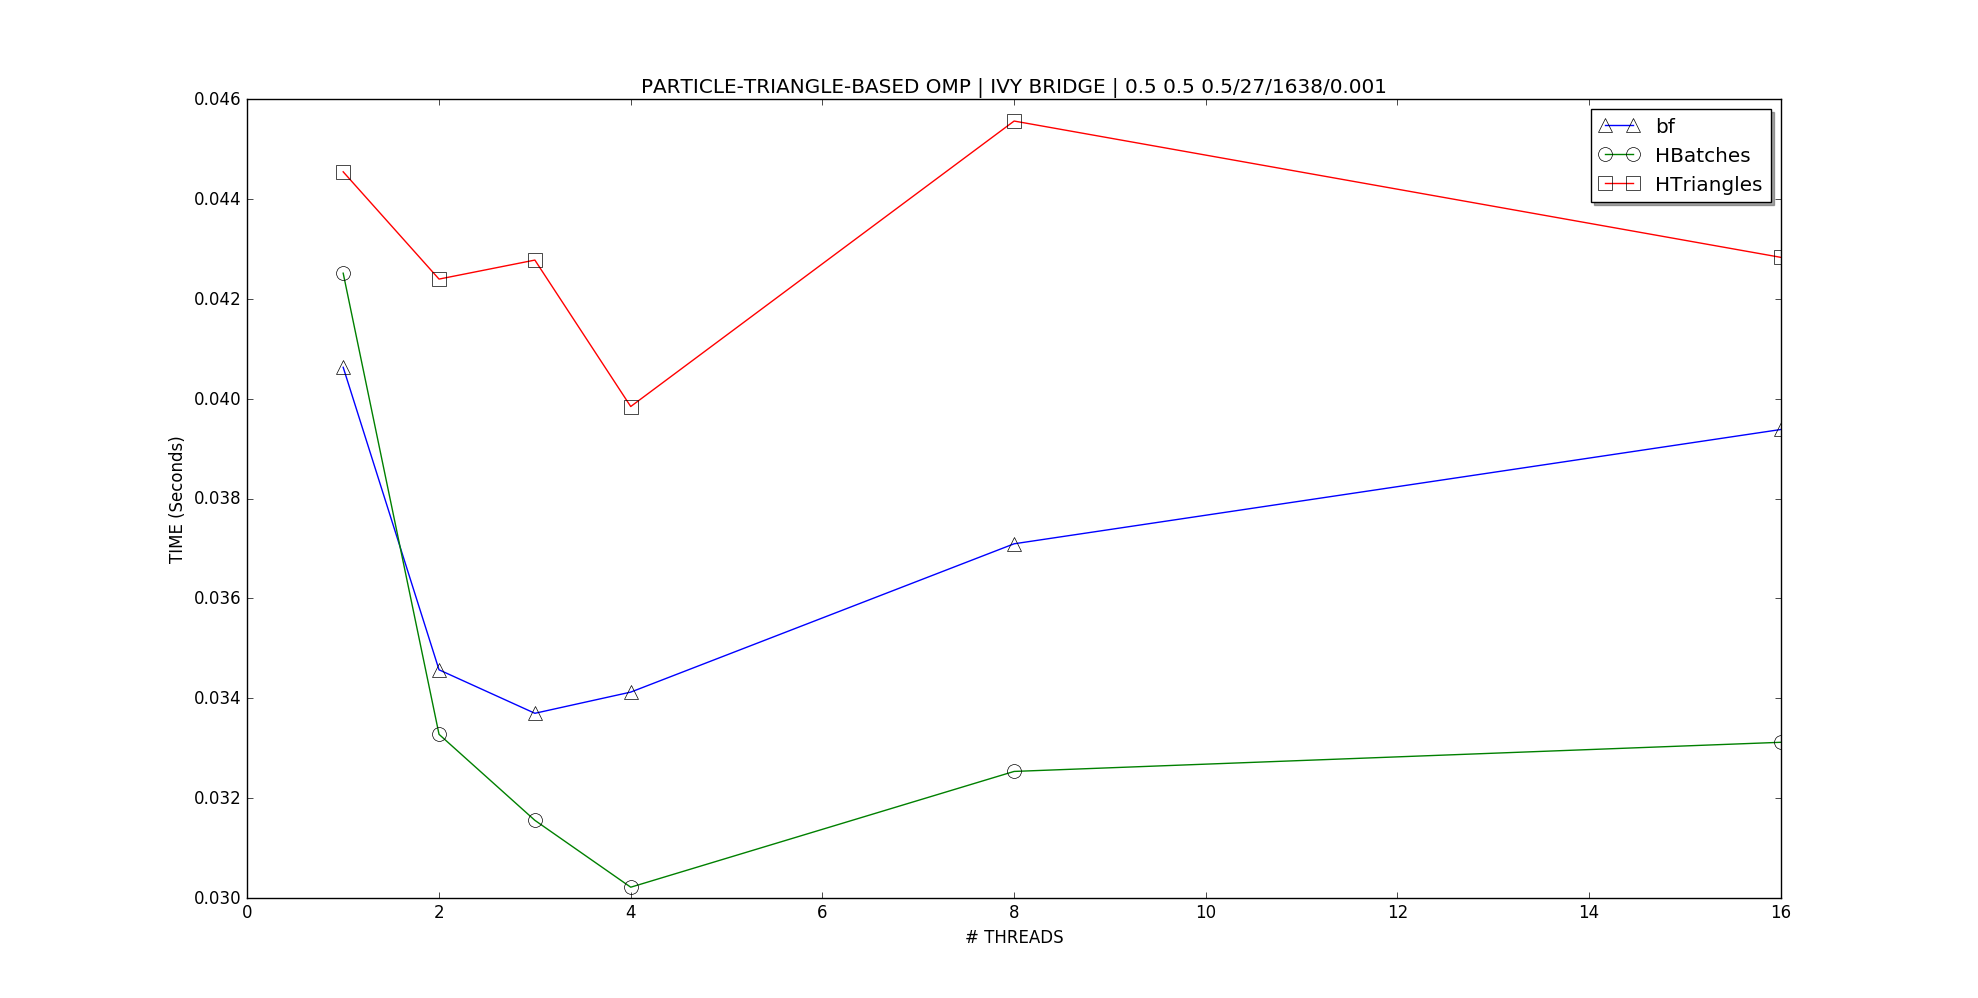
\includegraphics[width=0.7\textwidth]{experiments/random/omp/particle_triangle_based_x0.png}
  \end{center}
  \caption{Particle based nested shared memory brute force (bf)}
  \label{figure:particletriangle_omp}
\end{figure}

%Particle and Triangle parallelism nests both particle and triangle shared memory threads. The runtime to solution is slightly slower than particle-based parallelism due to overhead. 

%Nevertheless it has an impact on brute-force method as it scales smoother than particle-based only parallelism due to overhead. In this case hybrid-on-batches is also the fastest while the hybrid-on-triangle-pairs the slowest. 


At the highest level of shared memory parallelism is the grid cell-based multicore processing. It is based on the peano-framework that is using Intel TBBs to assign cells on threads. This has significant impact on the overall runtime performance in Figure \ref{figure:tbb_vs_serial} it is compared with plain serial execution. Number of threads on the x axis refer to TBB Cell-based threads, at the contact detection method level the computation is performed without shared memory parallelism but with vectorization enabled. For the specified experiment in Figure {} we observe no cell-based thread scaling but only reduction of time to solution. But when we increase the problem size further (figure \ref{figure:tbb_scaling}) we see that cell-based parallelism scales and it enhances execution time. 

\begin{figure}[htb]
  \begin{center}
    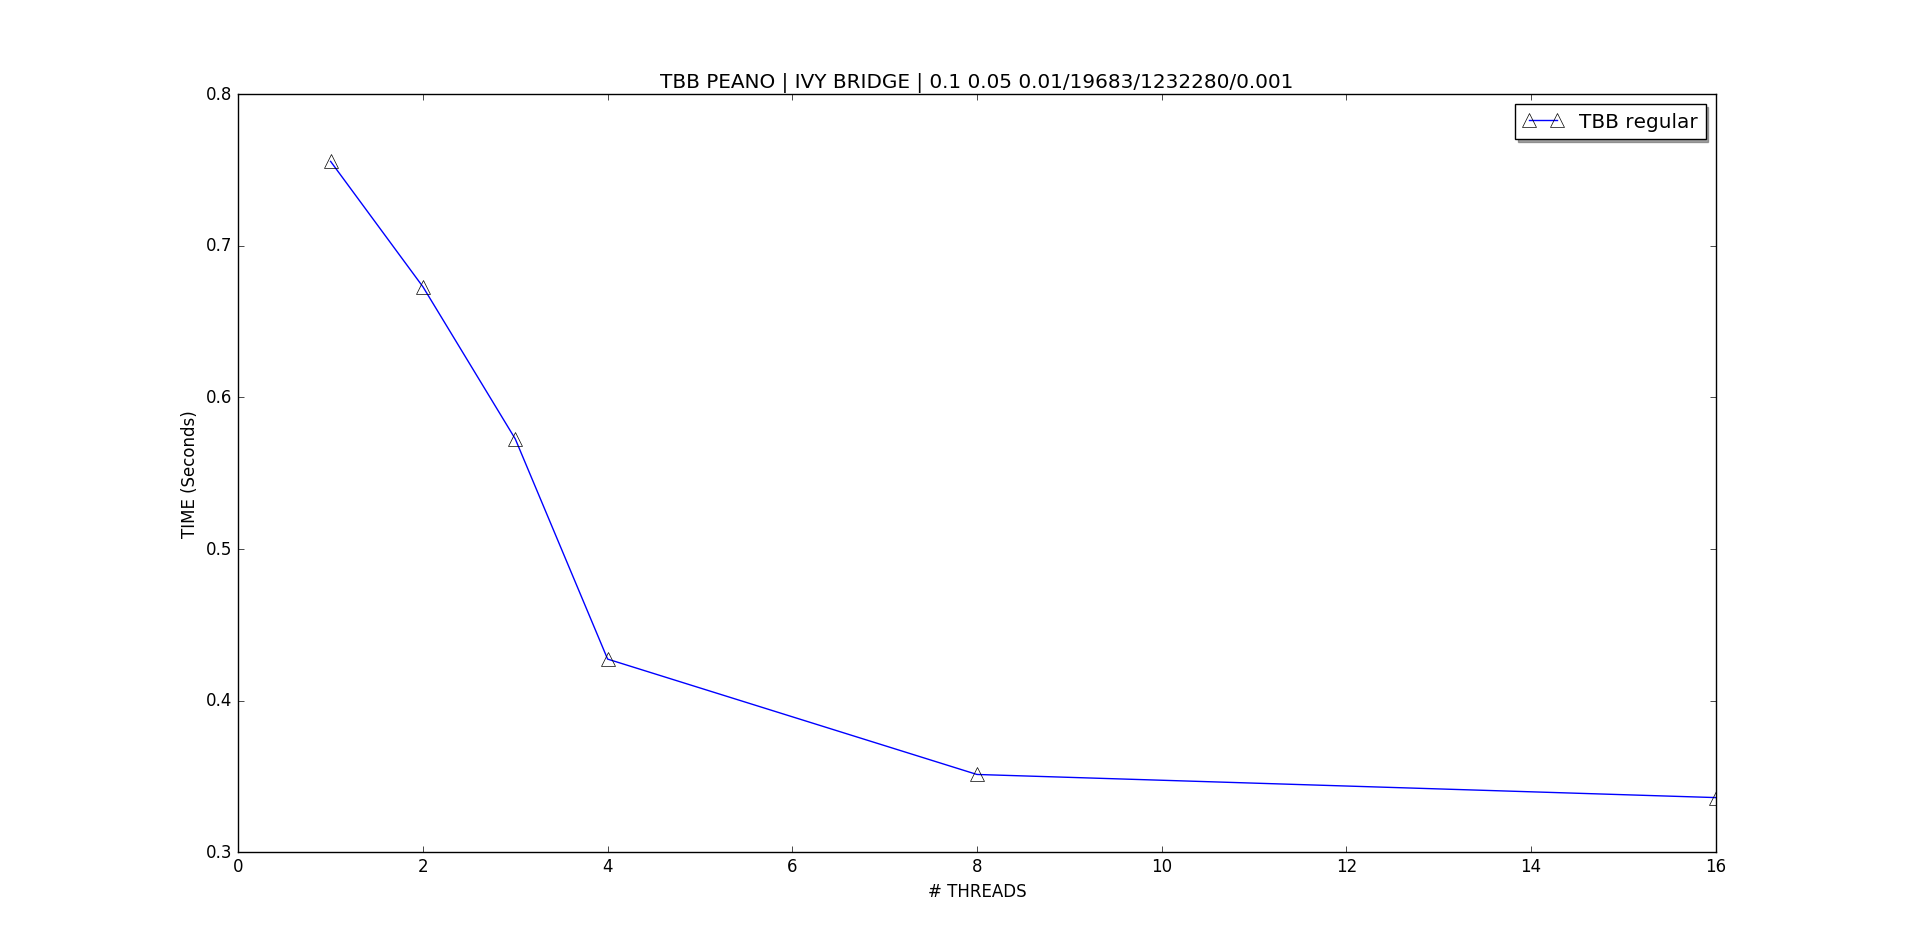
\includegraphics[width=0.7\textwidth]{experiments/random/omp/tbb_regular_x2.png}
  \end{center}
  \caption{Cell based parallelism on Peano compared to serial runs using Intel TBB}
  \label{figure:tbb_scaling}
\end{figure}

Overall shared memory parallelisation yield good speed ups both for hybrid and brute force using adaptive grids with triangle-based parallelism show good time-to-solution For large problem sizes the combination of cell-based plus triangle-based parallelism using hybrid-on-batches is the preferred option. Additional speedup can be gained if spheres are used as a filtering bounding box stage to our triangle-to-triangle contact detection.

\clearpage 

\subsubsection{Distributed Memory}

We scale the computation with the Message Passing Interface (MPI) \cite{Forum:1994:MMI:898758} for distributed memory computation. We study synchronous and asynchronous modes of data exchange and how two communication strategies can be exploited to increase performance and minimize computation. The algorithm is performed in four stages; At stage one, data migration assigns the sub-domains to MPI instances. At stage two, we compute the distances to determine contact between particles. In stage four we accumulate the data and in stage four we perform time step integration.

The number of neighbours has severe implication on communication patterns between processes. It is an open question what are the performance implications on uniform octree-based grids versus the non-uniform kd-tree based decomposition. It is an area of investigation. On uniform grids information about the level of refinement is known a priori by the sub-domain boundary size, which has interesting implications on multiscale simulations. 

The triangles that overlap into a remote sub-domain due to the decomposition cuts are temporary copied to one or more sub-domains to perform a complete contact detection. In this section, we study MPI communication characteristics when we resolve data dependencies between the sub-domains caused by ghost triangles in order to maximize performance of distributed contact detection. We explore the implication of inter-process communication and local computational performance using two communication strategies that use asynchronous non-blocking communication.

\begin{algorithm}
1. Load balance triangles

2. Migrate triangles to MPI network using blocking communication

3. Initiate neighbourhood all-to-all asynchronous MPI send/receive

4. Wait for neighbourhood asynchronous communication to terminate

5. Contact detection 

6. Derive contact forces from contact points generated

7. Explicit time integration

\protect\caption{\label{alg7}Naive Asynchronous Data Exchange Pseudocode}
\end{algorithm}


When spatial decomposition finishes we migrate the data to the processors (Algorithm \ref{alg7} line 2) with blocking synchronous communication. At each time step the triangles migrate according to the DEM kinematics. In addition to migration, a local area data exchange is required to communicate the boundaries of the sub-domains that cut triangles at the boundary. 

The first strategy exchanges local data to all neighbours (Algorithm \ref{alg7} line 3).  The goal is to utilize the communication bandwidth while minimise communication administration
overhead. If the exchange does not reach the upper bandwidth limit then exchange of all data is faster than filtering out the ghost triangles, i.e. doing any preprocessing that finds out which triangle from a sub-domain might be required from a neighbour. Alternatively, we can send out only triangles
that overlap from one sub-domain into another sub-domain. This filtering of triangles is an $O(N)$ operation. As soon as MPI communication finishes, the algorithm invokes the existing contact
detection routines exploiting vectorised floating point operations with a single contact detection routine. Exchange of all local data to all neighbours significantly increases the number of triangles to be processed from $T_{local}$ to $(T_{local} * N_{ranks} * T_{remote})$ where $N_{ranks}$ is the number of neighbours of neighbours. The increase of triangles to be checked increases the total computation performed locally because of the redundant triangles.

The disadvantage of such a naive method is that total MPI wait (figure \ref{fig6}) for an all-to-all neighbour data exchange increases with the number of processes. The asynchronous communication wait time results to time wasted with idle processors. The method is potentially useful with decomposition schemes where all data exchange can be processed in the background, i.e. enough bandwidth is available.

\begin{figure}[!h]
\centering
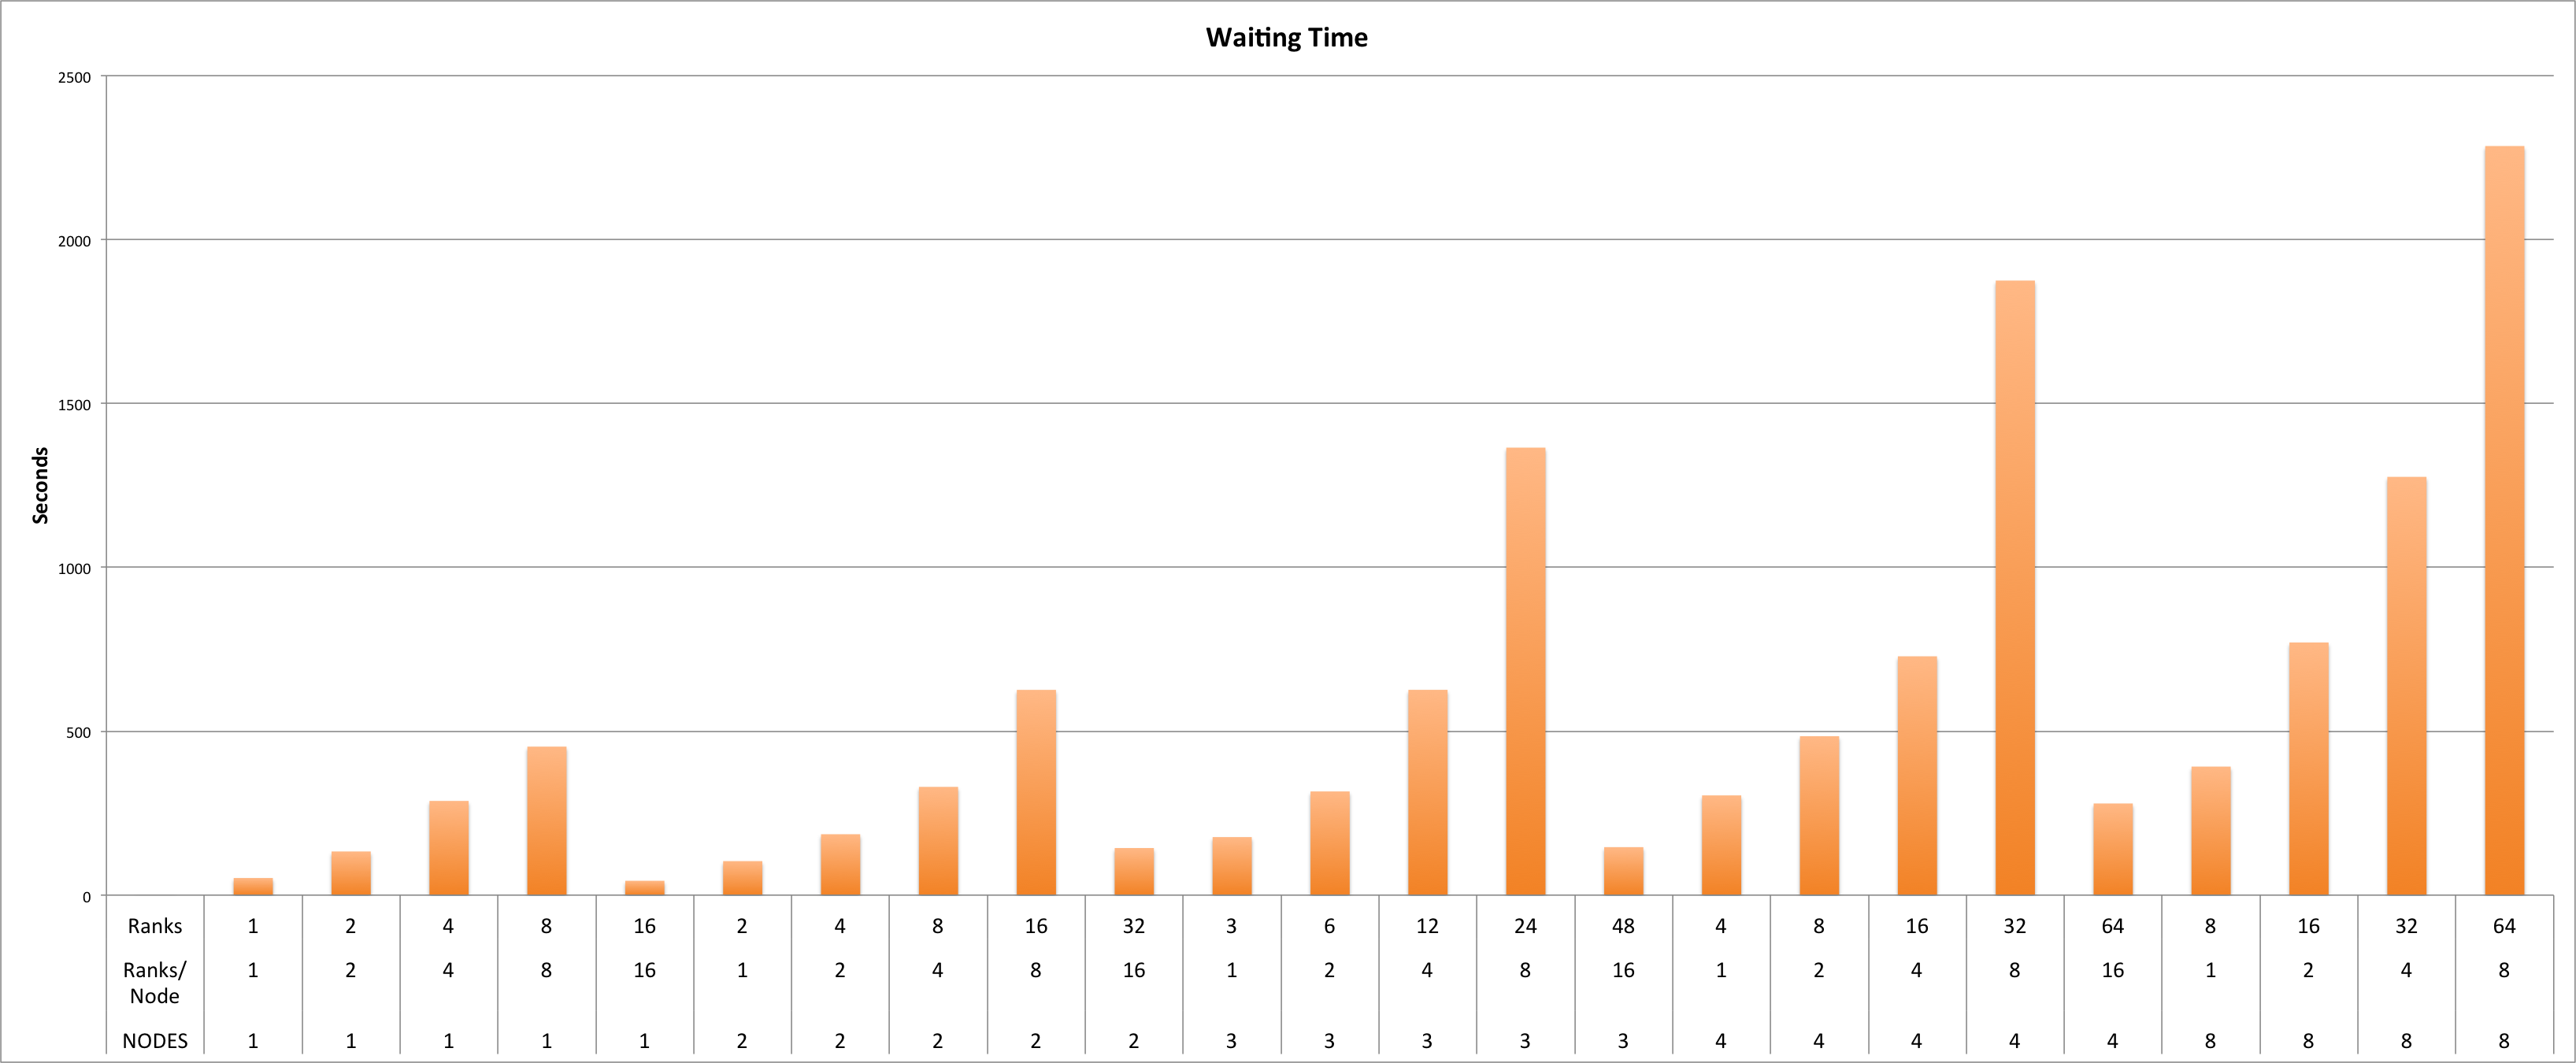
\includegraphics[width=1\textwidth]{wait} \protect\caption{\label{fig6}Waiting time (s) per MPI rank/node for all to all neighbour data exchange over 1000 time steps (25 mil triangles, 10k non-spherical particles).}
\end{figure}

\begin{algorithm}
1 Load balance triangles

2 Migrate triangles to MPI network using blocking communication

3 Search overlapping ghost triangles to send

4 Initiate neighbours asynchronous MPI send/receive

5 ~~~~~~Local contact detection

6 ~~~~~~Retrieve required ghost triangles from neighbours

7 ~~~~~~Local against to remote ghost triangle contact detection

8 Wait for neighbourhood asynchronous communication to terminate (No Real Wait)

9 Derive contact forces from contact points generated

10 Explicit time integration

\protect\caption{\label{alg8}Overlapping Asynchronous Data Exchange Pseudocode}
\end{algorithm}

The second strategy filters out local ghosts from the data structure and sends them to the overlapping neighbouring processes. Using the spatial decomposition information, we find the specific processes/boundary cells that the triangle bounding box overlaps. In this strategy we minimize data exchange at the cost of a filtering overhead and the allocation of buffers in memory. The method aims to minimise the waiting time of MPI processes by overlapping concurrent computation over communication. As shown in Algorithm \ref{alg8} line 5 local contact detection is executed as soon asynchronous MPI communication is initiated overlapping communication. A second contact detection is initiated to determine contact between local and remote ghost triangles at line 7. The strategy is advantageous as neighbour waiting is always zero as long as local contact detection takes longer than the transmission of the data. As shown in Figure \ref{fig6} the waiting time is increased proportionally to the number of MPI ranks, enabling us to increase overlapping computation per process with larger number of processes.

\begin{figure}[!h]
\centering
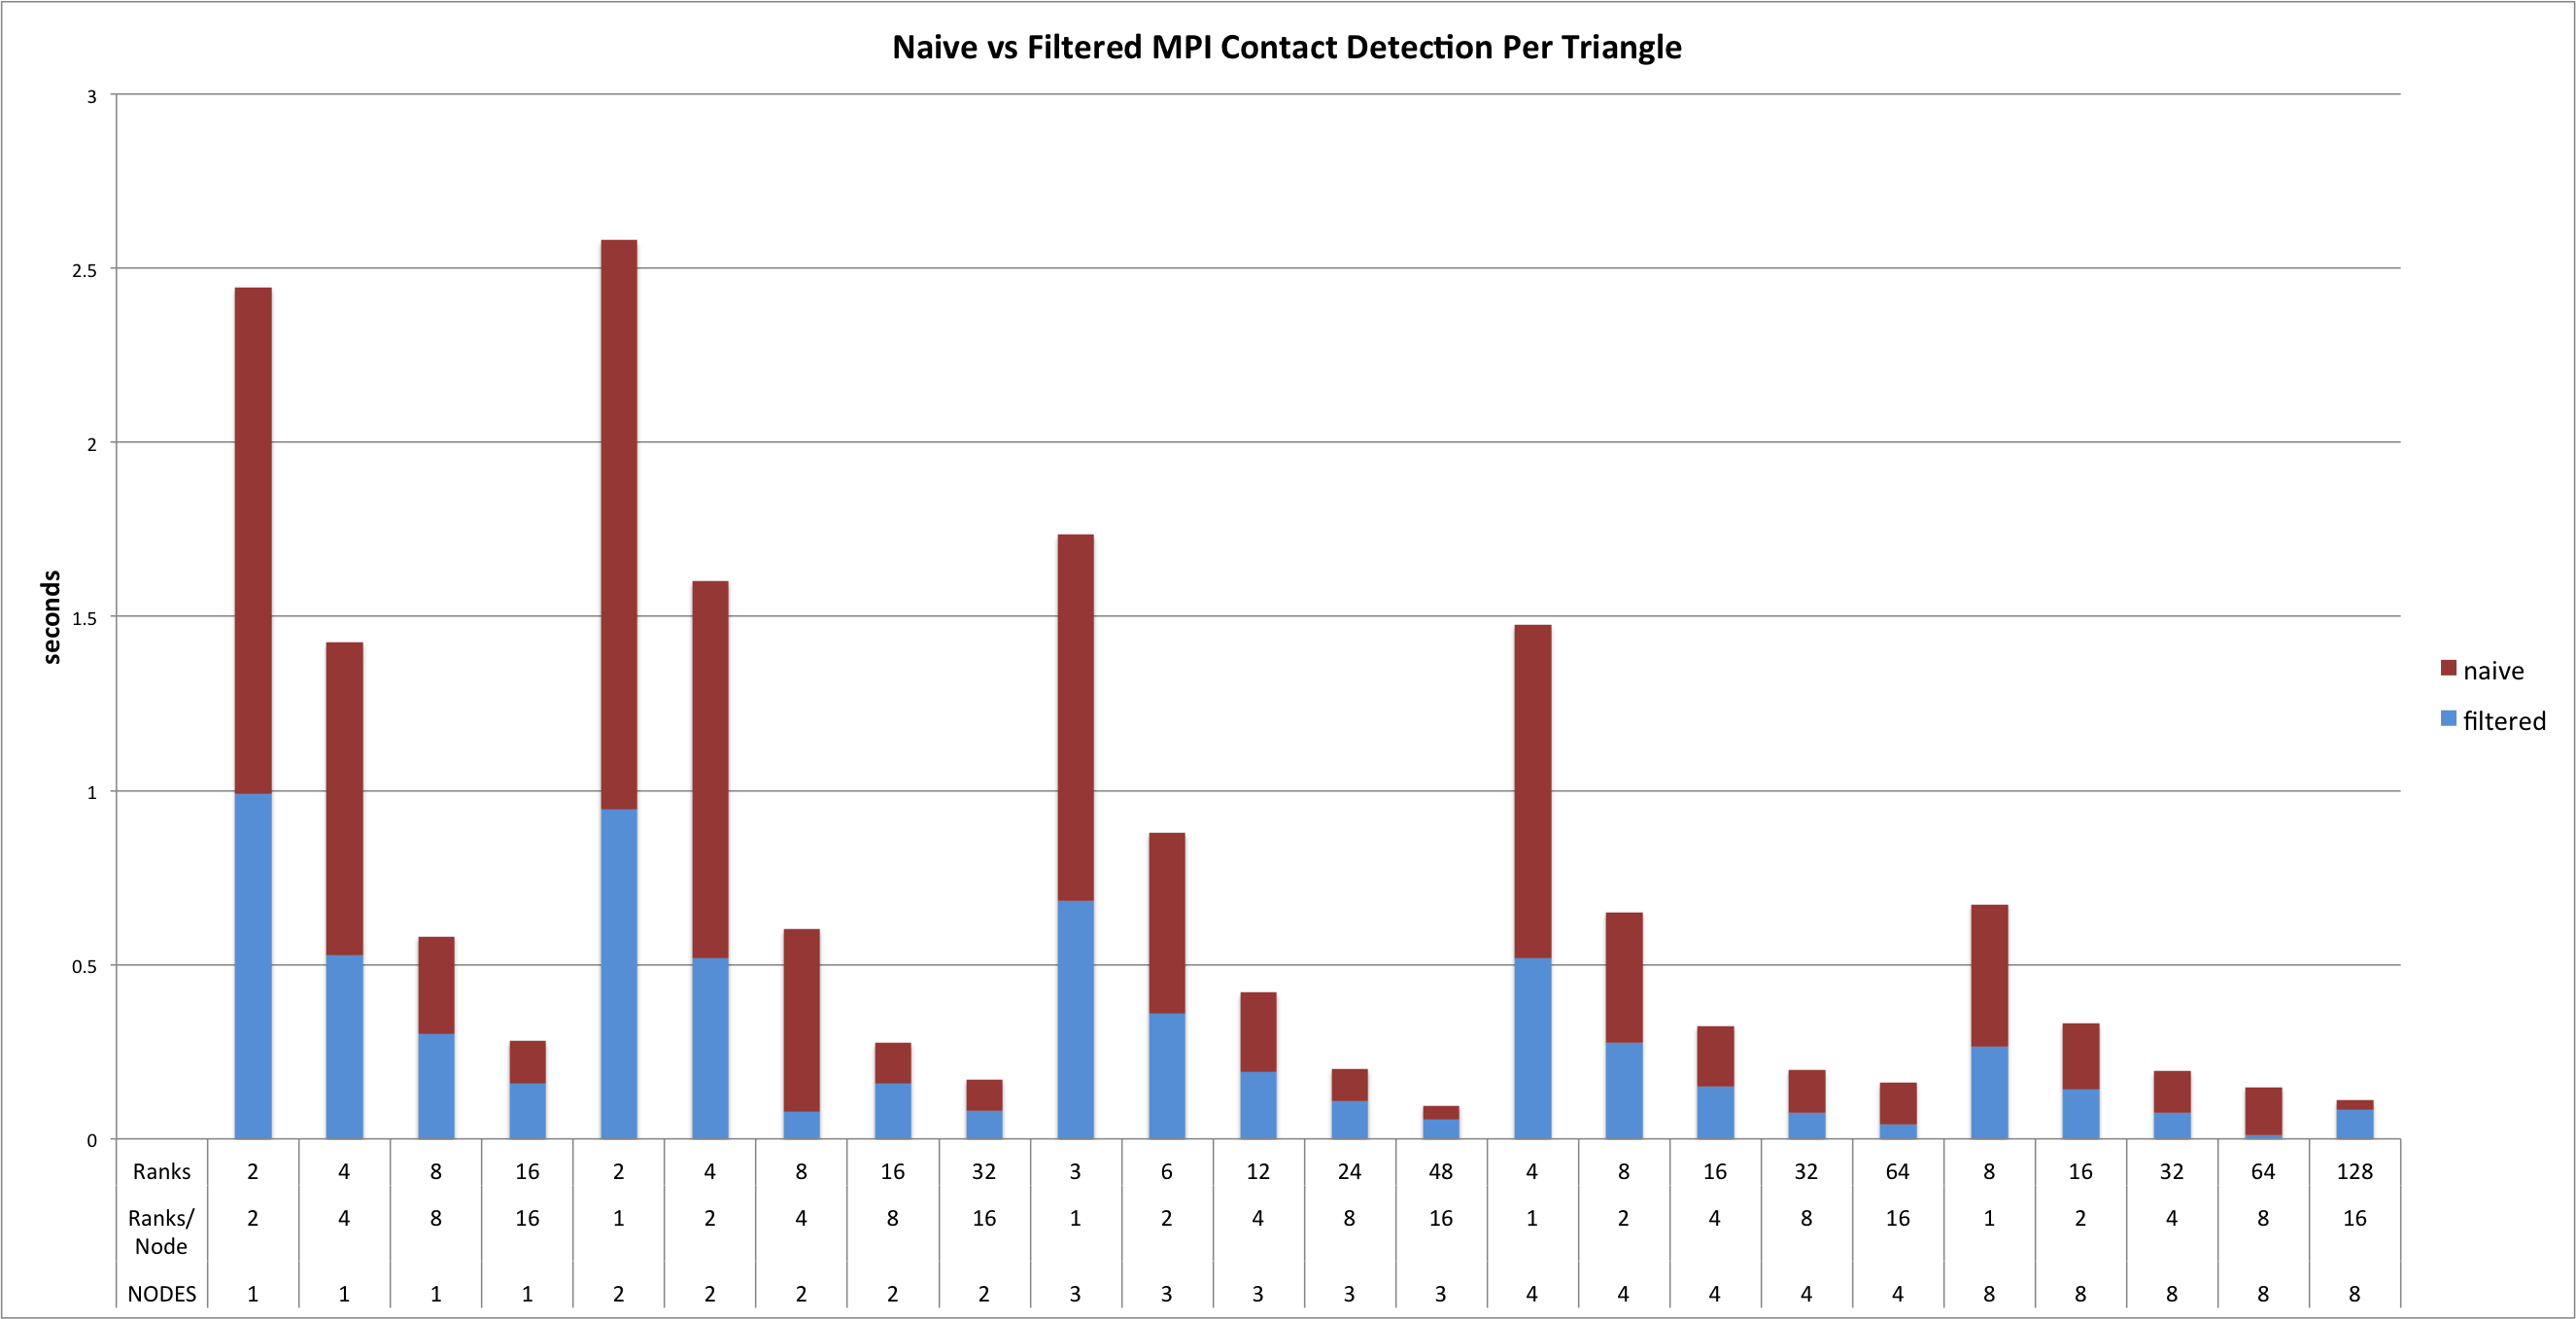
\includegraphics[width=1\textwidth]{mpi} \protect\caption{\label{fig7}Normalized naive vs filtered contact detection performance per triangle pair running on multiple nodes.}
\end{figure}

We measure both strategies to determine the performance of normalised computation per triangle. The result in Figure \ref{fig7} shows for each rank and compute node on the x axis, the time required to solve the distance of a pair of triangles. The blue bars show the average normalised time for the second strategy to process a triangle (filtering approach). The red bars show the difference between the overall naive communication time and the filtered method. The time is reduced linearly as the number of ranks increase. Figures \ref{fig6} and \ref{fig7} use Durham University Hamilton supercomputer that has per node 2 x Intel Xeon E5-2650 v2 (Ivy Bridge) 8 cores, 2.6 GHz processors, 64 GB DDR3 memory, 1 x TrueScale 4 x QDR single-port InfiniBand interconnect.

\subsection{Case Study}


\subsubsection{Hopper Flow}

\begin{figure}[!h]
\centering
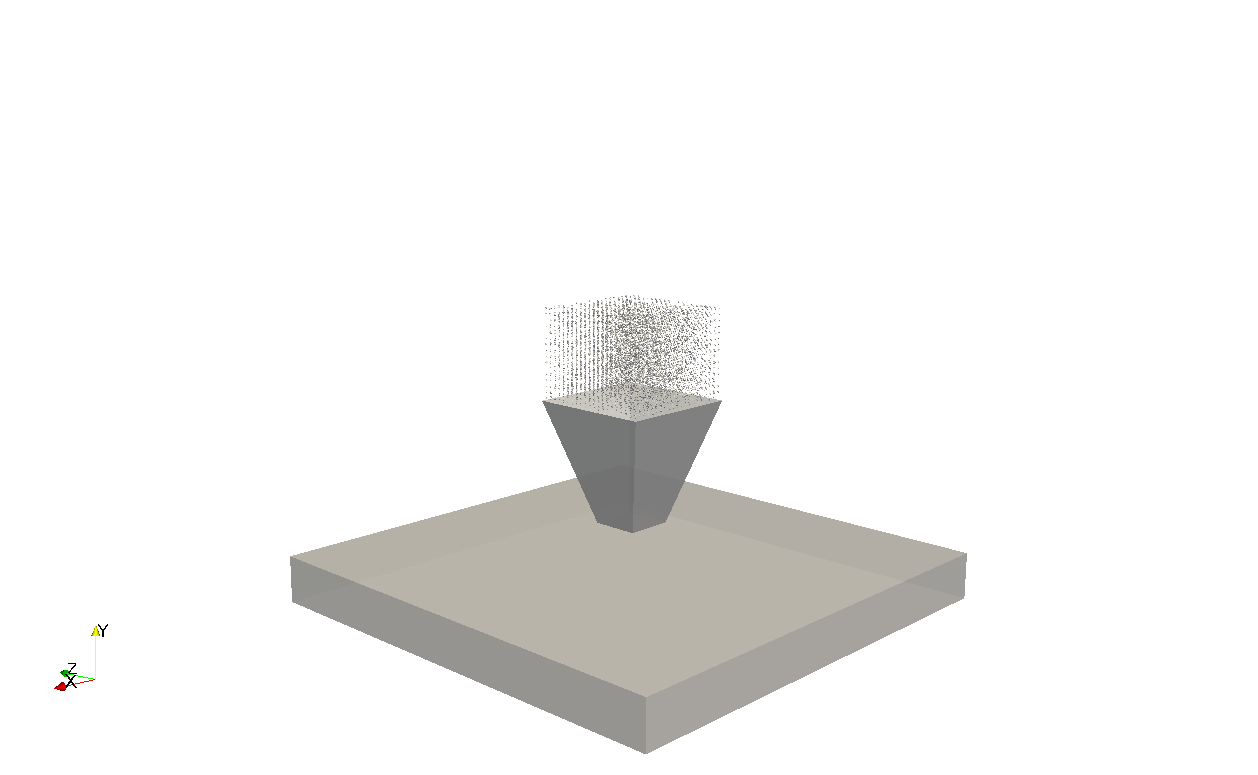
\includegraphics[width=0.7\textwidth]{sketches/hopper} \protect\caption{\label{hopper} Hopper structure and 120k non-spherical particles.}
\end{figure}

\begin{figure}[!h]
\centering
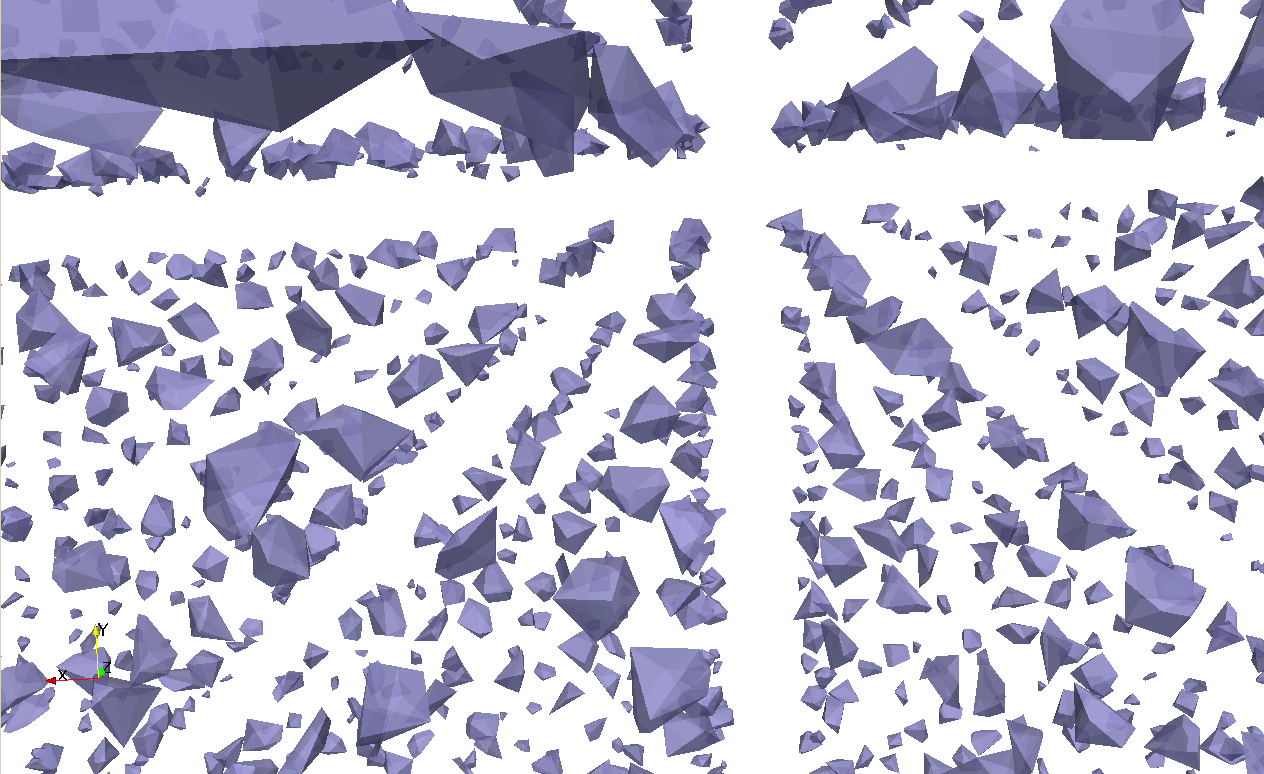
\includegraphics[width=0.7\textwidth]{sketches/granulatecloseup} \protect\caption{\label{hoppercloseup}Close up of non-spherical granulates.}
\end{figure}


\subsubsection{Seismic Shake}
\begin{figure}[!h]
\centering
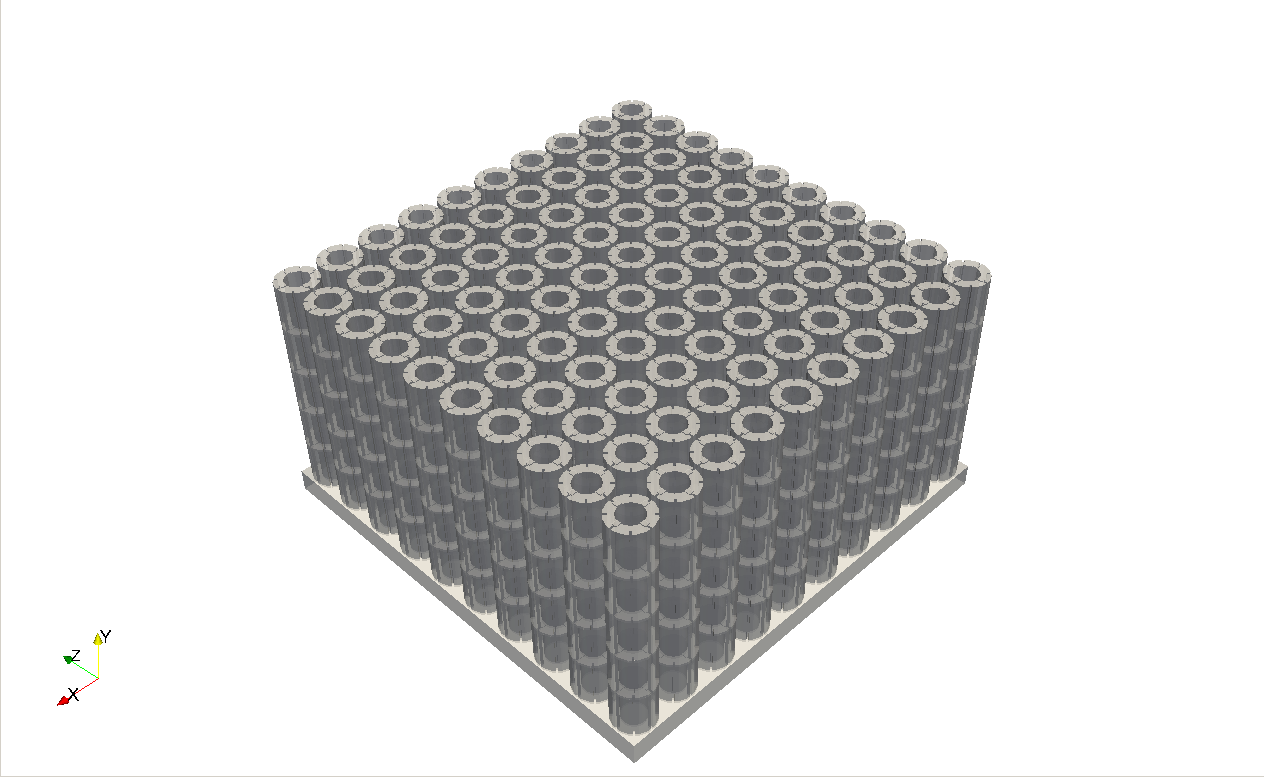
\includegraphics[width=1\textwidth]{sketches/nuclear} \protect\caption{\label{nuclear}Advanced gas cooled nuclear reactor array.}
\end{figure}

\begin{figure}[!h]
\centering
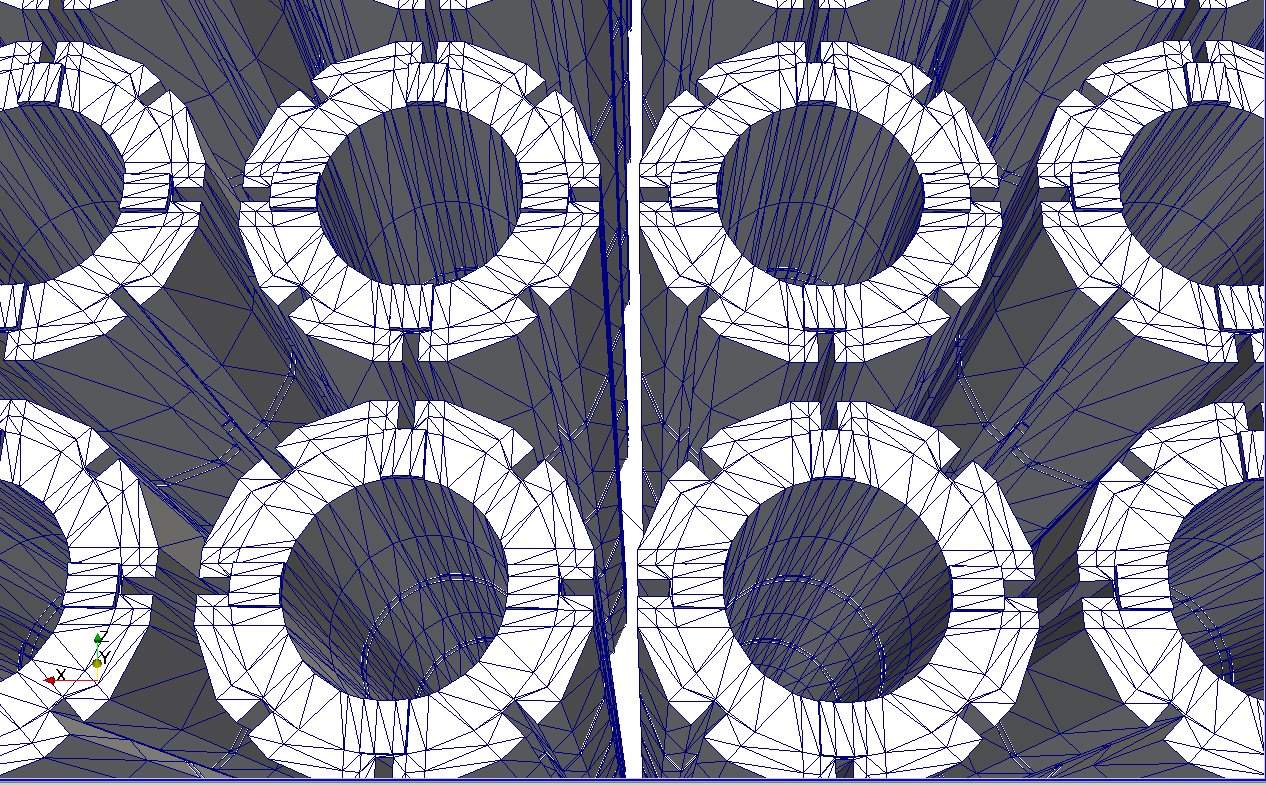
\includegraphics[width=0.7\textwidth]{sketches/nuclearcloseup} \protect\caption{\label{nuclearcloseup}Close up of meshed surface of nuclear graphite bricks of reactor.}
\end{figure}


\section{Critical Analysis}

\subsection{Open Issues}

In this research project, there are still some open issues that are to be addressed over the remaining duration. Firstly, i want to investigate multiscale particle communication on large scale distributed memory adaptive grids. Communication patterns that emerge in coarse-to-fine, fine-to-neighbour-coarse may affect scalability over multiple compute nodes. Another aspect of experimenting with the grid is load balancing where cells are weighted based on computational load in addition to space decomposition, weighted cells ensure that a densely meshed particle of fine cells is balanced with coarsely meshed particles on coarse cells. This has to be studied further to fully exploit multi grid capabilities. Other than scaling, if time allows, it would be helpful to benchmark all levels of computation with profiling tools. 

Another open issue is post processing of output data. Meta-data can become too large to be processed by one core depending on the number of time steps and number of particles. Visualisation is also not possible for large scale data without further processing or data decomposition. 

\subsection{Timetable}
\begin{figure}[!h]
\centering
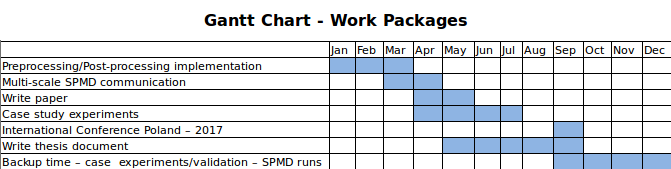
\includegraphics[width=0.8\textwidth]{chart} \protect\caption{\label{nuclearcloseup}Timetable for remaining time.}
\end{figure}

\subsection{Contribution}

Over the duration of this research several areas are covered and new insights are contributed. At the contact model level i introduce new numerical solvers for estimating the contact points by exploiting SIMD hardware. Building on top of the solvers and the background grid two hybrid schemes for shared memory DEM is introduced, one at the mesh level and one at the particle level both exhibit contrasting characteristics. 

At the grid level, we introduce a linked-cell approach to DEM to reduce the complexity O(n) of the overall computation. We store data at the vertex of the grid and combined by the reluctant adaptivity it pays off computationally. Multiscale particle communication over the grid will also be interesting contribution in computational DEM.

\subsection{Overall Assessment}

\vspace{5mm}
\begin{itemize}
\item Completed since last report: grid/spacetree implementation of DEM, shared memory benchmarks, interaction model (moment of inertia, rotations, material properties, damping, static and rolling friction), some preprocessing
\item New concepts: grid storage, grid shared memory, reluctant space adaptivity, adaptive time step size
\item Open questions: multiscale communication, benchmark of distributed memory
\end{itemize}

Overall the project covers all areas of large scale DEM overlooking into state of the art HPC aspects of other large scale numerical models. We investigated aspects of contact mechanics, kinematics, low level programming, parallel computation and that helps to fully integrate parallel computation with numerical modelling. Awareness of current state of the art implementations by other research groups also works as a reference to my own work.I believe that overall the research does not replace DEM model but instead could be useful as an augmentation library for contact detection for large scale DEM. The code library is very modular at every computational stage and particles elements can easily accommodate additional elements i.e. Reuleaux triangles.   
 
\subsection{Acknowledgments}
This work has been sponsored by EPSRC (Engineering and Physical Sciences Research Council) and EDF Energy as part of an ICASE studentship. This work also made use of the facilities of N8 HPC provided and funded by the N8 consortium and EPSRC (Grant No. N8HPC{\_}DUR{\_}TW{\_}PEANO). The Centre is co-ordinated by the Universities of Leeds and Manchester. We also thank University of Durham for the supercomputing resources and technical assistance. All underlying software is open source and available at: https://github.com/KonstantinosKr/delta.

\bibliographystyle{plain}
\bibliography{./papers}

\end{document}







